%-----------------------------------------------------------------------------
% Template for AIMS Rwanda Structured Masters Research Project
%
% The fonts, linespacing, numbering, page styles, order
% of  Title/Abstract/TOC/Body/{Appendices}/Acknowledgements/References 
% are prescribed as the AIMS house style.
%
% Do not change them or add to it without getting approval first.
% Essays are not accepted if they do not follow house style.
% This is in preparation for your Masters/PhD where the university
% will be much more strict on the house style.
%
\documentclass{aimsessay}
\usepackage[utf8]{inputenc}
\usepackage[round]{natbib}
%
%-----------------------------------------------------------------------------
% To use external packages for specific needs, 
% get approval before adding them here (they
% should not override general AIMS house style and layout).
%
% Examples:
%
% For Arabic
%\usepackage{arabtex}
%\usepackage{utf8}
%\setcode{utf8}
% For tables:
\usepackage{booktabs} % \toprule, \midrule, \bottomrule
\usepackage{array}    % \newcolumntype
% 
% For figures:
\usepackage[below]{placeins} % use \FloatBarrier in the body
% \usepackage{float}  %"H" placement spec, for **really here** (i.e. not float)
\usepackage{caption} %many figures in one figure (note subfigure and subfig are deprecated)
\usepackage{subcaption} %many figures in one figure (note subfigure and subfig are deprecated)
%
% For code and algorithms
\usepackage{moreverb}   % \verbatimtabinput
% For links and hyper references
\usepackage{hyperref}
\urlstyle{same}
% \usepackage{listings} % more flexible and complicated 
                        % than moreverb and algorithm
% 
% Others
% \usepackage[all]{xy} 
 \usepackage{sagetex}
% \usepackage{siunitx} % to typeset numbers, units, align decimals in tables.
% \usepackage{dcolumn} % less flexible but maybe faster than siunitx above.
% \usepackage{mathtools} % More maths, e.g. \mathclap.
\usepackage{epstopdf}
\usepackage{psfrag}
\usepackage{graphics}% Others may be landscape, longtable, algorithm, algorithmic, etc.
\usepackage{lineno} % This package together with lineno.sty numbers every line. Makes it easy for edditing.

% Numbers lines
\linenumbers
% 
% ----------------------------------------------------------------------------
% An AIMS Essay can use the sectioning commands "\chapter", "\section",
% "\subsection". No "\subsubsection", "\paragraph", etc. They are disabled.
% 
% For Theorems and such, use the environments defined here:
% \begin{thm}...\end{thm} (or "lem", "defn", etc)
% 
% We put the number to the left of the Theorem heading.
\swapnumbers 
% 
% Theorems are in italics.
\theoremstyle{plain}
\newtheorem{thm}[subsection]{Theorem}
%
% Rest is not in italics.
\theoremstyle{definition} 
\newtheorem{lem}[subsection]{Lemma}
\newtheorem{cor}[subsection]{Corollary}
\newtheorem{conj}[subsection]{Conjecture}
\newtheorem{pro}[subsection]{Proposition}
\newtheorem{exa}[subsection]{Example}
\newtheorem{defn}[subsection]{Definition}
\newtheorem{rem}[subsection]{Remark}
% 
% If you have no theorems, but a lot of equations, maybe the
% following two lines are good. Beware of corresponding Equation
% and Example numbers though! Number equations by sections.
% 
\numberwithin{equation}{section}
%
%-----------------------------------------------------------------------------
% Abstracts are usually written in English, with a version in your
% mother tongue underneath.
%
% French, Twi, Arabic, Malagasy, etc. students use normal LaTeX
% for special characters, for example \'{e}
%
% Amharic students use LibreOffice to write Amharic,
% export and include a figure.
%
%\begin{RLtext}    
%Here is where the arabic text goes.
%You can just type it with an arabic keyboard
%\end{RLtext}\\
%-----------------------------------------------------------------------------
 
% Your own command shortcuts can go here
% keep them clearly separate from other sections of the preamble
% It is good style to have only a few of these so that
% we can read one another's code. If you have too many, 
% then your code does not compile in someone else's template easily,
% and it makes it harder to read. These definitions are only
% meant for very often-used commands to save typing; Examples:
%
%\newcommand {\be}{\begin{equation}}
%\newcommand {\ee}{\end{equation}}
%\newcommand {\C}{\mathbb{C}} % Complex
%\newcommand {\Z}{\mathbb{Z}} % Integers
%\newcommand {\R}{\mathbb{R}} % Real
%\DeclareMathOperator{\sech}{sech} % declaring new math operators like \sin.
%  
%-----------------------------------------------------------------------------
% Title & Author
% On this page you must have NO full-word capitalizations, bold, or colour. 
% All AIMS essays per year have the same title page.
% In English your family name is written last, i.e. Firstname LASTNAME
% English Capitalization, not as in some Francophone countries where
% you write LASTNAME, Firstname.
% Put your AIMS email address only please, for consistency,
% not gmail or some other webmail address.
\title{The Title}
% Your name must be in CAPITAL with no comma, 
% and the Family name comes last.
\author{By\\ [1cm]
Alice Irankunda  (alice.irankunda@aims.ac.rw)\\
% Igbo, French students, put your special characters above.
% Arabic students can add their name in Arabic letters below, 
% after the english one
% Uncomment the next four lines and edit the name
%%%%%%%%%%%%%%%%%%%%%%%%%%%%%%%%%%%                  
%\begin{RLtext}    
%سشمششة شمثهنعة
%\end{RLtext}\\
%%%%%%%%%%%%%%%%%%%%%%%%%%%%%%%%%%
% Amharic students speak to Jan about how to add your name in your own alphabet.
% Everything here is prescribed; do not enter bold or ALL CAPS here,
% it will not be accepted.
%African Institute for Mathematical Sciences (AIMS) - Ghana\\
% Example1
 Supervised by Dr.Yabebal FANTAYE 
% University of Stellenbosch, South Africa
% Example2
% Supervised by Doctor Ingrid Rewitzky
% University of Stellenbosch, South Africa
%{\small Supervised by: Title Firstname Lastname}\\
%{\small Institute of Supervisor, Country}%
% Don't put the department, it becomes too long.
}
\date{{\small June 2017}\\ [0.5cm]
  {\scriptsize\it AN ESSAY PRESENTED TO AIMS RWANDA IN PARTIAL FULFILMENT OF THE REQUIREMENTS FOR THE AWARD OF MASTER OF SCIENCE IN MATHEMATICAL SCIENCES}\\%
  \vspace{3cm}{
\includegraphics[scale=.3]{images/aimsrw_logo.png}}}
%-------------------------------------------------------------------------
\begin{document}
%\selectlanguage{english}
\pagestyle{empty}
\maketitle
% All other files are included via \input. 
% To compile in texmaker while viewing any of those
% without having to switch back, use
%   Options > Define Current Document as 'Master Document'
% To not have to close a PDF, remove viewpdf from quickbuild 
% and open the PDF (once) manually: it will auto-refresh or with control-r
% 
%-------------------------------------------------------------------------
% The abstract is the first thing we want to see. No acknowledgements or 
% dedications here. Fetch the abstract from a separate file.
% Please write it in English and in your mother tongue.
% An abstract should be less than half a page, so that both abstracts 
% (that is both languages) fit onto one page.
% We number roman numerals until the main body
\pagenumbering{roman}
%-----------------------------------------------------------------------------
% See the acknowledgement.tex file and follow the instructions there.
\chapter*{DECLARATION}
\addcontentsline{toc}{chapter}{Declaration}
This work was carried out at AIMS Rwanda in partial fulfilment of the requirements for a Master of Science Degree.

I hereby declare that except where due acknowledgement is made, this work has never been presented wholly or in part for the award of a degree at AIMS Rwanda or any other University.

\vspace{1.5cm}
%%Please type in your fullname according to the order given and include your electronic signature here%%
Student: AMBO AMANDURE Jean-Médard  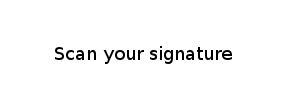
\includegraphics[height=1.5cm]{images/signature.png}

\vspace{1.5cm}

%%For the supervisor: Please type in your fullname according to the order given and include your electronic signature here%%
Supervisor: Jan Hązła 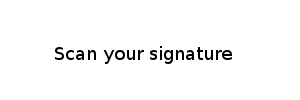
\includegraphics[height=1.5cm]{images/signature1.png}


\newpage

\chapter*{ACKNOWLEDGEMENTS}
\addcontentsline{toc}{chapter}{Acknowledgements}
% Don't change anything above this.
% We do not number this or add it to the contents!
% Overly long acknowledgements are not professional.


This research could not be achieved without the spiritual and intellectual support of several persons.
%First of all,  I am grateful to the God for his goodness.

First of all, I am highly indebted to African Institute for Mathematical Sciences for  the tremendous  financial support. Without this support,  this research and this master degree would not have been possible.

I would like to thank my supervisor Dr Jan H{\k{a}}z{\l}a for his helpful comments, remarks, encouragements and for introducing me to this interesting topic of research. Besides my supervisor, a thank you to all my teachers.

I would like to express my gratitude towards  my darling spouse, my children, my parents and members  of my family for their unfailing support and assistance. My absence was difficult to support. But you have endured. Thank you again.

My thanks and appreciations also go to my classmates for their kind cooperation and friendship. By this, my thanks also to the staff of African Institute for Mathematical Sciences.

Last but not the least, I am also grateful to my friends who have supported me along the way.

\newpage
\chapter*{DEDICATION} 
\addcontentsline{toc}{chapter}{Dedication}

This is optional.

% Abstracts are usually written in English, with a version in your
% mother tongue underneath
\chapter*{Abstract} 
\addcontentsline{toc}{chapter}{Abstract}
% Don't change anything above this.

A short, abstracted description of your essay goes here. 
It should be about 100 words long. But write it last.

An abstract is not a summary of your essay: it's an abstraction of that. 
It tells the readers why they should be interested in your essay but summarises all
they need to know if they read no further.

The writing style used in an abstract is like the style used in the rest of your essay: concise, clear and direct. 
In the rest of the essay, however, you will introduce and use technical terms. In the abstract you should
avoid them in order to make the result comprehensible to all.

You may like to repeat the abstract in your mother tongue.

% At a unviersity like Stellenbosch you *must* produce an abstract in Afrikaans for your masters.
% At AIMS you are encouraged to repeat the abstract in your mother tongue
% French, Igbo, Mlagasy, etc. just write it using LaTeX's special
% characters.
% Arabic students see the arabic.tex file for an example
% Amharic use openoffice and export from there and import a figure here.
% Where the words do not exist put the English work in italics, or use mathematical symbols.





% Don't go typing out the contents.
\tableofcontents
\newpage
% We switch to arabic numerals here where your page count starts
% Essays must be 35 pages long *starting here* and up to and including
% the conclcusion. It does not include the acknowledgements or references.
% 
% Figures may differ between topics, but they are not there
% to fill the pages -- they must add meaning.
% In general most figures should be 0.8 times the width of the page
% (perhaps wider in total when two or three columns of figures)
% See the example in chapter one for defining that. Be *consistent*
% in your presentation of information.
\pagenumbering{arabic}
\pagestyle{myheadings}
%-----------------------------------------------------------------------------
% Each chapter goes in a separate file
% Chapter titles are just examples
% Always have a question
% Note the Case Pattern used at AIMS
\chapter{Introduction}

Zika virus is a member of the Flaviridae family
and the flavivirus genus, it is related to other mosquito borne viruses such as Dengue Virus, Yellow-Fever (YFV) virus  and West Nile virus \citep{doi}.The Virus originates from the Zika forest of Uganda and the first case was first isolated in 1947 from a rhesus monkey in the forest. Then later in 1954 a human was diagonised with the virus in Nigeria,\citep{2015zika}. Since then the virus has spread to different parts o the world. 
\begin{figure}[h!]
\centering
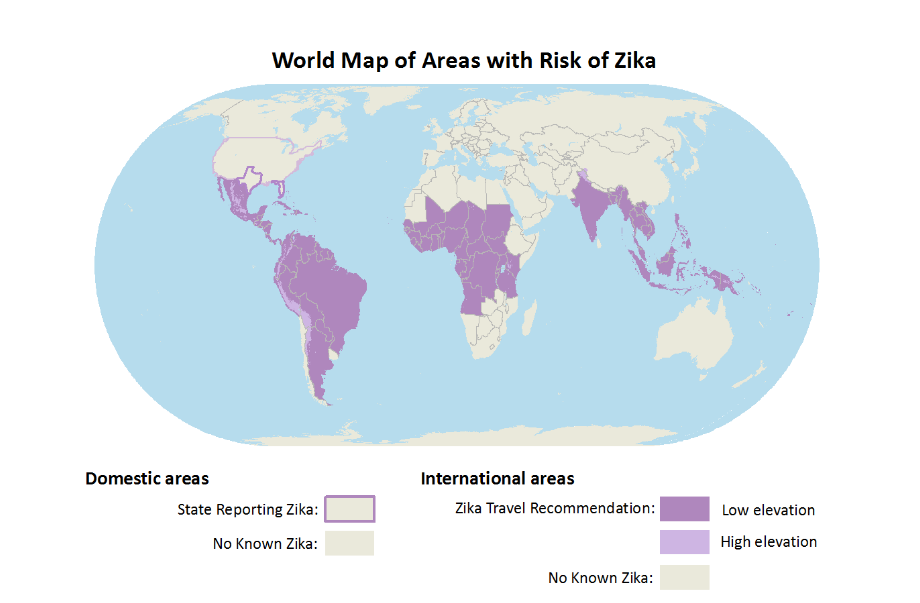
\includegraphics[scale=0.5]{images/map_zika.png} 
\caption{Counties with Zika Virus: Source CDC}\label{fig 1}
\end{figure}


Zika Virus is mainly spread by Aedes mosquitoes, when the Mosquito bites an infected person it carries the pathogen and when It bites an infected person it also it leaves the pathogen in them. Other ways of by which the virus spreads include, Blood transfusion, Unprotected Sex With an infected person and From mother to child, infected mothers can pass on the virus to their unborn children \citep{musso2014}.

\cite{musso2015}, shows that some of the symptoms are papular rash,fever,arthritis or arthralgia. In addition , headache, joint pain and red eyes are common symptoms of Zika virus. \cite{simoes2016zika} state adds that pregnant mothers who are infected with Zika during usually have child bearing defects. The Zika virus affect their foetus and development of the baby. Babies can face a range of neurologic sequelae suc as intellectual disability, hearing loss, vision loss, and seizures. These problems can range from mild to severe, are often life-long \citep{rasmussen2016zika}.

There is no known vaccination to prevent or treat for Zika virus. Prevention measures can be taken to prevent the spread of the virus. Preventing mosquito bites, this can be done by sleeping under a mosquito net, using mosquito replant, spraying mosquitos inside and outside among others. Another measure of prevention of Zika virus is practising safe sex and avoiding travelling to areas with high prevalence of Zika virus. Drugs for the systems of Zika are administered to patients as a way of treating Zika infected people because of the luck of a vaccination for the virus.


The spread of Zika virus has resulted in Zika epidemics in some part of the world as can be seen in figure \ref{fig 1} above. This cause a worry as the effects of an epidemic are more diver stating and if not controlled can affect the whole country region and World at large. 


 
 Mathematical models for disease transmission have been used to link biological processes of disease transmission and emergent of dynamics of infections at the population level. Researchers try to understand the environmental, biological  and behavioural infectiousness of a disease .
 
  Environmental infectiousness depends on geographical factors of an infected person. Some pathogens cannot survive inside or outside in given conditions. Thus some diseases or infections spread faster in certain weather conditions\citep{grass}. Understanding the timing and causes of seasonality offers important insights into how parasite–host systems interact how and when parasite control measures should be applied, and how disease risks will respond to anthropogenic climate change and altered patterns of seasonality \citep{altizer}. These factors must be captured in the models.
  
  Biological infectiousness depends on the pathogen's life cycle and the individual or host immune system. Some individuals have strong immune system against certain infections. This on the slows down the propagation the infection. On the other hand pathogens that live outside also affect the transmission dynamics of the infection.  The interaction of the genetic determinant of disease propagation in the pathogen and host is important in building model for the transmission dynamics of infectious diseases.
  
Behavioural infectiousness depends on the interaction behaviour of an individual. The contact pattern of the person affect how the individual is likely to propagate   the disease. Depending on the nature of disease transmission, if a persons has a lot of contact they are more likely to spread the disease to more people compared to one who has few contacts \citep{johnson2001sexual}. Contact in this context implies any interaction likely to result in the transmission of an infection.

The susceptibility of and individual largely depend on biological, environmental and behavioural factors of an individual. For example one's contact pattern, immunity and the environmental conditions will highly affect the probability of contracting an infection.

Epidemiologist together with mathematicians have for years been involved in infectious disease modelling to understand the dynamics of the spread of the disease and to come with measures of how the spread can be controls. Recently there has been a growing interest in modelling the spread of Zika virus \citep{ku2016}.

Over a  century, Mathematical representation and analysis of infectious diseases has been the centre of  infectious disease epidemiology \citep{b2005}. Differential equation have been used in the modelling of the dynamics of infectious diseases. They are base on the assumption of uniform mixing, that is everyone in the population has an equal probability of contracting an infectious disease \citep{kaplan2002emergency}.
Compartmental Mathematical models have been used to describe the transmission dynamic of Zika Virus \citep{gao2016}.

Mathematical modelling of infections diseases, started by the works of Daniel Bernoulli in \cite{bernoulli1760essai},in the quest to model the spread of small box and possible eradication. A century later the modelling become well established. The modelling of infectious disease dynamics is important for science and public policy among others. The models for infectious disease is helpful for prevention and planning the control of the spread of these disease. Policy makers use the information generated from the models in their policy formulation. In science it opens up new field of science and is vital in the study and development of drugs.

The dynamics of infectious disease propagation are modelled as dynamical system. A dynamical system is a system that evolves with time over a state space according to a fixed rule. Thus let $\mathbb{X}$ be a state space $\mathbb{T}$ set of times and $\mathbb{R}$ rule that specifies how the state evolves with time. the rule is a function that whose domain is $\mathbb{X} \mathbb{T}$ and co domain $\mathbb{X}$ that is,
\begin{equation*}
\mathbb{R}: \mathbb{X} \mathbb{T} \longrightarrow \mathbb{X}.
\end{equation*}

The population is characterized as $S(t)$, $E(t)$,$I(t)$ and $R(t)$ . Where $S(t)$ is the number of individuals susceptible but not infected at time $t$, $E(t)$ is the number of people exposed or infected but not infectious at time $t$, $I(t)$ is the number of infected and infectious people at time $t$ and $R(t)$ is the number of people removed from the ability of being infected.Removal is carried by either immunization,death,recovery from the disease. The epidemiological models can be classified as Susceptible,Infected and Recovered (SIR) , Susceptible Infected (SIS or SIS) , Susceptible -Exposed - Infectious and Removed (SEIR)  and any other intermediate category can be added.

The SIS model assumes that there is no immunity after recovery used to model infections where once a person recovers they become susceptible again for example infectious like flue. SIR model assumes that once a person recovers they become immune to the infection for example chicken pox. The SEIR assumes that onnce a person get becomes infected they do not  become infectious intermediately hence the intermediate compartment for exposed. 

The independent variable in the compartmental model is the time $t$ and the rates of transfer between compartments are expressed mathematically as a result models are formulated initially as differential equations. The most epidemic models are built on the SIR proposed by \cite{m1925applications}. The system can be written as;


\begin{center}
\begin{equation} \label{eqn1_1}
\left\lbrace \begin{array}{ccl}
\frac{dS}{dt} &= &-\alpha S_{(t)} I_{(t)},\\
 \frac{dI}{dt} &=& \alpha S_{(t)} I_{(t)} - \gamma  I_{(t)}, \\
 \frac{dR}{dt} &= &\gamma  I_{(t)},
\end{array} \right. 
\end{equation}
\end{center}

 with assumptions that there is homogeneous mixing in the population. That is the rate of new infections is proportional to the current numbers of susceptibles and infectives in the population. Which the main assumption deterministic models are built on. Deterministic population  models are models where the behaviour of the population of determined completely by history and the rules which govern the model. In formulating these models , in terms of derivatives of the sizes of the compartments and it is assumed that the number of members in each compartment is differentiable with time. This assumption is tenable only when the disease outbreak has been established  but not valid at the beginning of a disease out break when they are few infectives. When they are a few out breaks the number of infectious depends on random contacts of between small number of individuals.
 
 On the other hand Stochastic models are obtained by setting by adding a random variable called noise to the transmission dynamics of deterministic models.These random fluctuations may impact the evolution of the infection. Unlike deterministic model which assume homogeneous mix , an assumption which only holds in small populations. It is quiet unlikely that all people in will be equally susceptible to the disease and effective in spreading it \citep{ball1985deterministic}. A stochastic model can be further be described as a model in which the distribution of the length of the infectious period as allowed to have any distribution that can be describe by its Laplace transform \citep{addy1991generalized}.
 
 Lets an SIR compartmental model, for $t > 0$, $S(t),I(t),R(t)$ is the number of individuals in susceptible, infectious and removed. $N(t)$ the total number of particles at time $t$. The Poisson process, which is the underlying structure basic to the class of stochastic models and all Markov chain processes\citep{greenwood2009stochastic}. The individuals enter each compartment at random times and the initial fixed values , $S(0)$,$I(0)$ and $R(0)$ are fixed for some $\lambda > 0$. Letting $\beta$ to be the average number of  contacts an infectious person makes per unit of time that take leads to infection. The probability of a susceptible individual moving from compartment S to compartment I in the time interval $\left[ t,\triangle t \right]$ that is  S $\rightarrow S-1$ and I $\rightarrow I + 1 $ is $ \beta$ S I $ \triangle t + o (\triangle t)$. If it is assumed the an infected person recovers at the rate $\gamma$ hence the probability of an infected person moving from infected to recovered over an interval $\left[ t,\triangle t \right]$  given by $\gamma I_{t + \triangle t} -o (\triangle t)$ .It is known that,
 \begin{align*}
 N_t = S_t + I_t + R_t
 \\ \Rightarrow  R_t = N_t - S_t - I_t
\end{align*}  
Which implies that knowing $S_t,I_t$ is knowing $R_t$. Hence the model becomes an $S_t,I_t$ and thus the stochastic dynamical system can be written as;
 \begin{align}
 P((S_{t + \triangle t}, I_{t + \triangle t} - (S_t ,I_t) = ( - 1,1)) =  \beta S I  \triangle t + o (\triangle t).
 \\ P (((S_{t + \triangle t}, I_{t + \triangle t} - (S_t ,I_t) = ( 0,-1)) = \gamma I_{t + \triangle t} -o (\triangle t).
 \end{align}
 

Graph theory has over the years grown and has found its application many fields. A graph also known as a network   can be  defined as triple $G = (V,E,f)$ where $V$ is a finite set of nodes $E \subset V \oplus V = \left\lbrace e_1,e_2,\dots ,e_m \right\rbrace$ is a set and f is a mapping which associates some elements of $E$ to a pair of elements of $V$ \citep{estrada2012structure}. 

Some network properties that can be used to describe networks or graphs.A network is said to be connected if between any pair of node there exists a path. In modelling disease spread a connected network is one in which an infection could travel from one person to any other person in the network through some steps. Another property that is used to describe networks is distance. Distance between any two nodes in a network is defined as the length of the shortest path by each a node can be reached. This can be summed up as the average distance taken over al, pairs of individuals , which gives the idea of the typical distance between nodes in a network or the diameter of the graph which is the largest distance taken over all pairs \citep{chung2002average}.

The number of of neighbour is denoted by $k$ is known as the degree of connectivity. Looking at the entire population (space), the quantities  give a connectivity distribution. The degree is also describe as a mean and denoted by $<k>$.

Some other measures that can be used to describe a network measure are cliquishness, clustering coefficient, transitivity  coefficients and mutuality examine the extend to which the neighbourhood individual have a common neighbour,  leading to the appearance of triangles in  in the network.

 The concept of random graphs was first introduced by \cite{erdodblac1959ldquo}. A graph or network is said to have a small world property if it has a high clustering coefficient and a small average path length. This means that every node in the network can be connected with another using only few connections \citep{estrada2015first}. In 1967 there was an experiment carried out by Milgram, in which randomly selected individuals living in Kansas and Nabraska were asked to send a latter to someone in Boston, directly if they knew the person or through someone they new personally. It was found that the latter was sent through an average of 6 people and it was discovered that some acquaintances of an in individual were feeding the letter into back into the cycle \citep{travers1967small}.

A random graph can be defined as , given a $N$ number of vertices edges between them are drown such that between any pair $i,j$ there is an edge with uncorrelated probability $p$ \citep{newman2002random}. For example in \ref{fig:randomgraphs}, there are 3 random graphs with 10 vertices, with a probability of nodes $i,j$ being connect being 0, 0.5 and 0.8 in figure \ref{fig:a} \ref{fig:b} and \ref{fig:c} respectively. A random network model can exhibit the small world network property, it has an average degree $z= pN$. Random networks have a a low clustering coefficient $ c = \frac{z}{N}$ \citep{newman2003structure}.

Classical models are built on an assumption of full mixture , random networks on the other hand are said to be well mixed. Thus they have a much lower epidemic threshold than the expected real world population \citep{witten2007simulations}.
\begin{figure}[h]
    \centering
    \begin{subfigure}[b]{0.3\textwidth}
        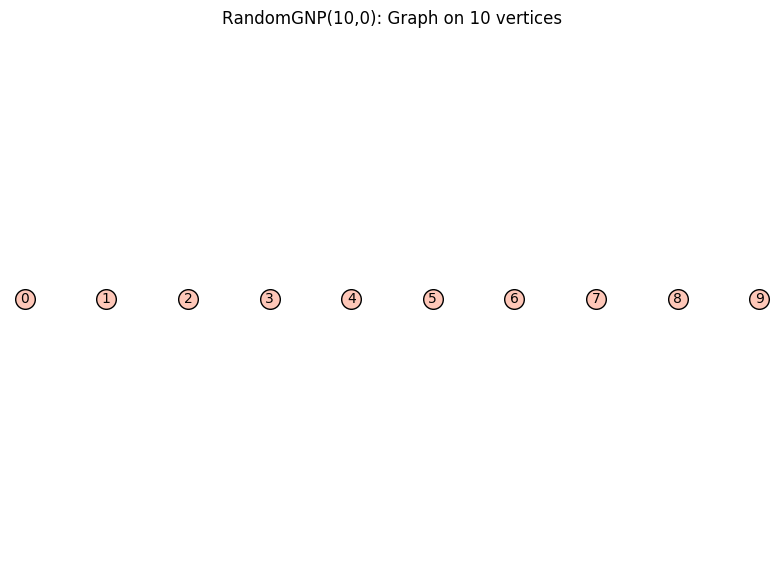
\includegraphics[scale=0.3]{images/rgraph2.png} 
        \caption{ $p =0$}
        \label{fig:a}
    \end{subfigure}
    ~ %add desired spacing between images, e. g. ~, \quad, \qquad, \hfill etc. 
      %(or a blank line to force the subfigure onto a new line)
    \begin{subfigure}[b]{0.3\textwidth}
        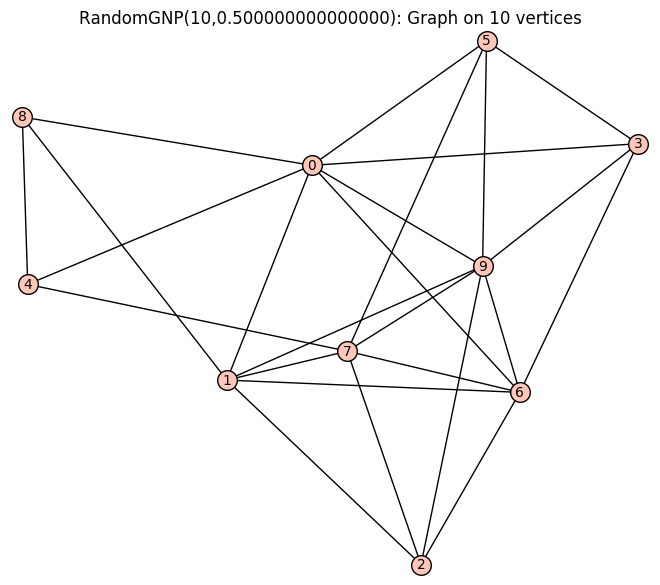
\includegraphics[width=\textwidth]{images/rgraph1.png}
        \caption{$p=0.5$}
        \label{fig:b}
    \end{subfigure}
    ~ %add desired spacing between images, e. g. ~, \quad, \qquad, \hfill etc. 
    %(or a blank line to force the subfigure onto a new line)
    \begin{subfigure}[b]{0.3\textwidth}
        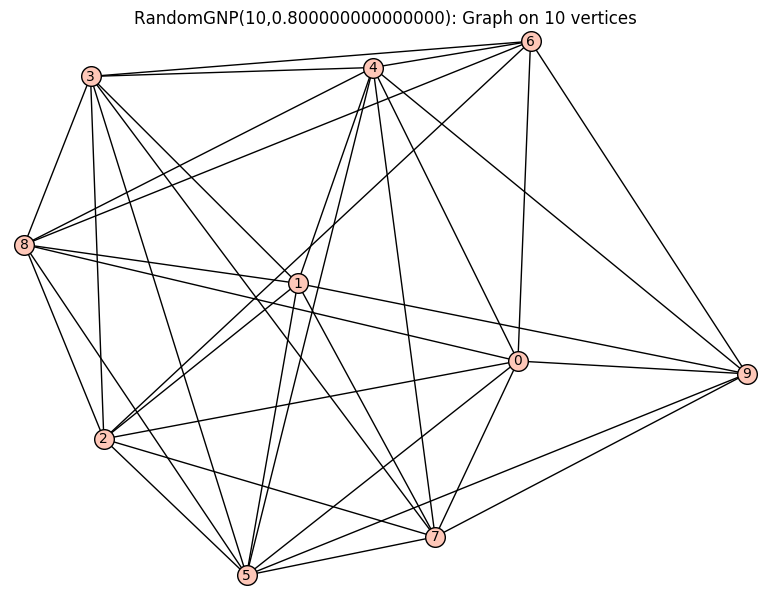
\includegraphics[width=\textwidth]{images/rgraph3}
        \caption{$p= 0.8$}
        \label{fig:c}
    \end{subfigure}
    \caption{Random Graphs}\label{fig:randomgraphs}
\end{figure}


In addition to Random graphs there are other networks on which epidemiology models have been built on   Watts–Strogatz, lattice,Barabasí–Albert, and power-law or “scale-free” \citep{witten2007simulations}. These networks have a small world properties except for the Barabasí–Albert network.The model have different network structures and network statistics, which is not the scope of this paper.


Regular lattices and random graphs have a long history of use in network theory and to model population structures,\cite{harris1974contact}  gives an example of classic lattice. Models built on latices assume that individuals are located as nodes on a regular lattice and connections are made of some collection of near neighbours or each node. For example people may be spread out such that connections are made to their four nearest neighbours, one on the left,right, up and down this is called a Neuman neighbours  or eight neighbours where four diagonal elements are added to the Neuman neighbours and this is called the Moore neighbour hood \citep{lloyd2006infection}.To avoid the effect of the nodes at the end not being connected the last and first neighbours are made neighbours.

The main difference between a random graph and lattices is that interactions are local, that is individuals are only related to their neighbours. Where as in random networks the connections are made are global, that is connections are made without taking spatial locations of an individual into consideration. 


Small world networks  were first introduced by Watts and Strogatz as an intermediate between the regular lattice and randomly rewiring certain proportions $p$ of the network links\citep{watts1998collective}. The small world networks allows for random contacts across the network. That is in addition to near neighbours as in a regular lattice, each node has a random distant neighbour connected to it \citep{watts1998collective}.

 
 on the other hand assume that one is more likely to spread the disease to someone in their family, someonewho lives near the, or someone you they. It combines this sort of clustering in the graph with a probability to model the spread of disease as a dynamical system \citep{newman2001random}.


In this research we will compare the traditional epidemiological model based on Random network assumption and the Small world networks to model the population Dynamics in the spread of Zika Virus. This infection of of Zika virus will be modelled using the SEIR compartmental model based on the two assumptions of transmission. Then real life data will be fit on both models to validate each model and to test which on is better.

 % Introduction is usually a chapter itself.
\chapter{On the Hales-Jewett theorem}

In this part, some notions about Hales-Jewett theorem are presented. Firstly, we start by some basic notions on arithmetic progression, which are important for understanding the next point. After, we introduce some elementary notions about  Van der Waerden’s theorem and  Szemerédi's theorem. We highlight that  Van der Waerden's theorem is a particular case of Szemerédi's theorem. Ultimately, we present the two forms of Hales-Jewett theorem and link these one to the two first theorems.

\section{Arithmetic progression}


\begin{defn}
Let $a_1, a_2, \ldots, a_n, \ldots$ be a sequence of numbers.  

This sequence of numbers form an \textbf{arithmetic sequence} if every term of this sequence is obtained by adding a constant to the previous term.
\end{defn}
The constant is simply the difference between two consecutive terms.

If $a_1$ and $a_n$ represent the first and the $n-$th term of a sequence, and $d$ the constant, then the general term $a_n$ of this sequence is expressed as:

$$a_n=a_1+(n-1)d.$$

Knowing $a_m$ and the constant $d$, then $a_n$ can be expressed as:
 
$$a_n=a_m+(n-m)d.$$

\subsection{Arithmetic progression of length k}


Let $a$ and $d$ be two fixed numbers.

An arithmetic progression of length k is an arithmetic progression of $k$ numbers of the form $a+nd.$ $a$ is the first term of the arithmetic progression, $d$ is the difference between two consecutive terms and $n=0,1, \ldots, k-1$, that is $k$ consecutive values of $n.$ 

We denote by AP$(k)$ or AP$-k$ or $k-$AP, the arithmetic progression of length $k.$


\section{Van der Waerden's theorem}

Before stating the Van der Waerden's theorem, let us introduce and define some concepts and notation.

A \textit{partition} of a set $A$ is a collection of nonempty and mutually disjoint subsets $A_i$ of $A$, such that  $A=\cup A_i$ and $A_i \cap A_j=\emptyset, \quad i\neq j.$ Thus, a partition is also a sequence $A_1, A_2, \ldots, A_n$ of mutually nonempty and  disjoint subsets of set $A$. $A_i$ are known as \textit{blocks}.

We denote by $\mathbb{Z}^+$, the set of positive integers.
Let $m \in \mathit{Z}^+$, we designate by $[m]$ the set $\{1,2, \ldots, m\}.$
%\Jnote{Use ldots instead of cdots}.

Let $X$ be a set and $r$ be a positive integer. We want to colour elements of set $X$ with $r$ colours. If $C$ represents the set of colours, then $|C|=r$ is the number of colours.

\begin{defn} An $r-$colouring of $X$ is a mapping $c \ : \ X \longrightarrow [r].$  \label{rcol}\end{defn}
\Jnote{Still a problem here: You should write \$r\$-coloring,
with - outside math mode.}


If $|X|=n$, then the number of $r$-colorings of $X$ is $n^r.$

%\Jnote{Better: ``the number of $r$-colorings of $X$ is''}

Let $Y$ be a subset of $X.$ $Y$ is \textit{monochromatic} when the restriction $c\restriction_Y$ is constant, that is   if $c(y)$ is the same for every $y \in Y.$

%\Jnote{For restriction better use \textbackslash restriction and write $Y$
  %in lower script, like this: $c\restriction_Y$.}

According to \cite{polymath2012new}, the Van der Waerden's theorem is stated as follows:

\begin{thm}[Van der Waerden]
For every pair $(k,r) \in \mathbb{Z}^+ \times \mathbb{Z}^+$, there exists $N_0 \in \mathbb{Z}^+$ such that for every $N \geq N_0$ and for 
every $r-$colouring of $[N]$ there is a monochromatic arithmetic progression of length $k.$  \label{vd1}
\end{thm}

%\Jnote{I think it is more consistent with other theorems to state this as:
  %``there exists $N_0$ such that for every $N \ge N_0$''}

We know that an $r-$colouring is a function called $c$ in definition \eqref{rcol}. So, in other words we can find at least one subset of $\{1,2,\ldots,N\}$ with $k-$elements such that all elements have the same colour and form an arithmetic progression of length $k$. That is, there exit
\Jnote{s/exit/exist}
$a$,  $d \ \in \mathbb{N}$ with $d\neq 0$ such that: $c(a)=c(a+d)=c(a+2d)=\ldots =c(a+(k-1)d)$ where $a, a+2d, \ldots, a+(k-1)d$ are elements of the subset.

This Van der Waerden's theorem can also be formulated using partition \citep{dransfield2004} as:

\begin{thm}[Van der Waerden]
For every $k, r \in \mathbb{Z}^+$ , there exists $N_0 \in \mathbb{Z}^+$ such that for every $N \geq N_0$ and for every partition $A_1, \ldots , A_r$ of $[N]$, there is $i$, $1 \leq i \leq r$, such that the block $A_i$ contains an arithmetic progression of  length $k.$   \label{vd2}
\end{thm}

Note that for this version a block in a partition can be empty. 

The existence of the number $N_0$ for which any $r-$colouring of the integer $\{1, \ldots, N_0 \}$ is certain to have a monochromatic subset of cardinality $k$ of which elements form an arithmetic progression was demonstrated constructively in 1927 by Bartel Leendert van der Waerden in \cite{van1927beweis}.

\cite{graham1974short} gave \emph{another} proof of this theorem. The book entitled "\textit{Purely Combinatorial Proofs of Van Der Waerden-Type Theorem}" written by \cite{gasarch2010purely} condenses  the proof of Van Der Waerden theorem.
\Jnote{Be careful with capitalization: it is
  ``Van der Waerden's theorem''.}

In this theorem, the difficult problem is to find the number $N$.
\Jnote{Rephrase this. Even showing that $N_0$ is not trivial
  (also correct typo $N->N_0$).}
The least such number $N_0$ is called \textit{Van der Waerden number} denoted as $W(k,r).$ In the rest of this chapter, we will use $W(k,r)$ or simply $W$ to denote the least Van der Waerden number instead of $N_0.$

The general expression of $W(k,r)$ is not known, but for some $k$ and $r$ there are exact values known or there are some approximations of the  lower or upper bound of $W(k,r)$  \citep{dransfield2004}.

$W(1,r), \ W(k,1)$ and $W(2,r)$ are known as \textit{trivial} Van der Waerden numbers. So, 
\begin{itemize}
\item $W(1,r)=1$:  the set of all subsets of a nonempty set contains necessary a singleton. A singleton forms an arithmetic progression of length $1$ where the difference between two consecutive numbers is $0.$ To form a monochromatic arithmetic progression of length $1$ by $r-$colouring a set, we need  a set of at least one element. 
\item $W(k,1)=k$: by colouring a set with one colour, we automatically get a monochromatic arithmetic progression of length equals to the cardinality  of the set.
\item $W(2,r)=r+1$: to obtain a monochromatic arithmetic progression of length $2$ by $r-$colouring a set, we need a set of at least $r+1$ elements.
\end{itemize}

For instance, let us find the Van der Waerden number $W(3,2)$, that is a $2-$colouring  of the set $[W(3,2)]$ such that there is a monochromatic arithmetic progression of length $3.$
\Jnote{Rephrase: ...that is $N_0$ such that every $2$-coloring of $[N_0]$
  contains a monochromatic...}

The value of $W(3,2)$ is greater than $8$ because for any $2-$colouring of $[n],\ n\in \{3,4,5,6,7,8\}$, we can find a $2-$colouring which does not contain a monochromatic arithmetic progression of length 3. For instance, the set  $\{1,2,\ldots, 8\}$ doest not contain a monochromatic  arithmetic progression of length $3$ by $2-$colouring the set  like in the table \eqref{van23}.

So, when $W(3,2)=9$ we always find a monochromatic arithmetic progression of length 3 for any $2-$colouring of $[9].$ The table \eqref{van23} shows one of the possibilities of colouring $\{1,2,3,4,5,6,7,8,9\}.$  If the ninth number is {\color{blue} blue}, then{ \color{blue}3, 6, 9}  form an arithmetic progression. If the ninth number is {\color{red} red}, then {\color{red}1, 5, 9} form an arithmetic progression. Therefore, by adding a ninth number and colouring it using any of the two colors, we always create  a monochromatic arithmetic progression of length 3.

\begin{table}[h]
\begin{center}
\begin{tabular}{ccccccccc}
\hline
1 & 2 & 3 & 4  & 5 & 6 & 7 & 8 & 9 \\ \hline
\color{red}R & \color{blue}B & \color{blue}B & \color{red}R & \color{red}R & \color{blue}B & \color{blue}B & \color{red}R  & \\
\hline 
\end{tabular} 
\end{center}
\caption{A $2-$colouring of $\{1,2,\ldots, 9\}$} \label{van23}
\end{table}

\Jnote{This example is now very well explained!} 

The table \eqref{vdn} presents the 7 exact non-trivial Van der numbers  (when $k\geq 3$) \citep{dransfield2004}.

\begin{table}[h]

\begin{center}
\begin{tabular}{|c|c|c|c|}
\hline 
$k \setminus r$ & 2 & 3 & 4  \\ 
\hline 
3 & 9 & 27 & 76  \\ 
\hline 
4 & 35 & 293 &   \\ 
\hline 
5 & 178 &  &   \\ 
\hline 
6 & 1132 &  &   \\ 
\hline 

\end{tabular}
\end{center}
\caption{The 7 exact non-trivial values of Van der Waerden numbers.} \label{vdn}
\end{table} 

As related previously, searching for the exact value of $W(k,r)$ remains a difficult problem.
\Jnote{s/difficult/open and then delete next sentence.}
By the way, it is an open problem. The number $W(k,r)$ becomes hard to find when the values of $k$ and $r$ increase. However, for some $k$ and $r$ there is an approximation of the lower or upper bound of $W(k,r)$ \citep{stevens1978computer, herwig2007new, beeler1979some, dransfield2004, brown2008bounds, rabung2012, kouril2008van}. The table \eqref{vdw1} summarizes these known lower bounds and includes the seven non-trivial Van der Waerden numbers known exactly.

\begin{table}[h]
\begin{tabular}{|c||c|c|c|c|c|}
\hline 
$\mathbf{k \setminus r}$ & \textbf{ 2 }& \textbf{3} & \textbf{4} & \textbf{5} & \textbf{6} \\ 
\hline  \hline
\textbf{3}  &	9	& 27 &	76 &	 \textgreater  170 &	  \textgreater  223 \\ \hline 
\textbf{4}	& 35 &	293  &	 \textgreater 1,048 &	 \textgreater 2,254 &	 \textgreater  9,778 \\ \hline 
\textbf{5}	& 178	& \textgreater 2,173 &	 \textgreater 17,705 &	 \textgreater 98,740 &	 \textgreater 98,748 \\ \hline 
\textbf{6}	& 1,132 &	 \textgreater 11,191 & \textgreater 91,331 &	 \textgreater 540,025 &	 \textgreater  816,981 \\ \hline 
\textbf{7}	&  \textgreater 3,703 &	 \textgreater  48,811 &	 \textgreater 420,217 &	 \textgreater 1,381,687 &	 \textgreater 7,465,909 \\ \hline 
\textbf{8}	&  \textgreater 11,495 &	 \textgreater 238,400 &	 \textgreater 2,388,317&	 \textgreater 10,743,258&	 \textgreater 57,445,718\\ \hline 
\textbf{9}	&  \textgreater 41,265 &	 \textgreater 932,745&	 \textgreater 10,898,729&	 \textgreater 79,706,009&	 \textgreater 458,062,329 \\ \hline 
\textbf{10}	 &  \textgreater 103,474&	 \textgreater 4,173,724&	 \textgreater 76,049,218&	 \textgreater 542,694,970 &	 \textgreater 2,615,305,384 \\ \hline 
\textbf{11}	&  \textgreater 193,941&	 \textgreater 18,603,731&	 \textgreater 305,513,57 &	 \textgreater 2,967,283,511 &	 \textgreater 3,004,668,671 \\ \hline 
\end{tabular} 

\caption{Some lower bounds and exact non-trivial values of Van der Waerden numbers $W(k,r).$} \label{vdw1}
\end{table}

The estimation of lower and upper bounds is also an open problem. There exist some expressions that bound Van der Waerden numbers.  Researchers are still looking for closer bound or exact general expression of these numbers.
 \cite{erdos1952combinatorial}, cited by \cite{dransfield2004} established an inequality for the lower bound for $W(k,r).$
\begin{equation}
\left[2(k-1) r^{k-1} \right]^{\frac{1}{2}} < W(k,r). \label{erdos}
\end{equation}

\cite{brk1968} found a better bound when $k-1$ is prime number  and for $r=2$. But these bounds still  require improvement. 
%\Jnote{Do not use symbols inside sentences,   write ``when $k-1$ is prime''.}
 \begin{equation}
 (k-1)2^{k-1}<W(k,2). \label{berlk}
 \end{equation}

For $p=k-1$, the expression \eqref{berlk} becomes:
 \begin{equation}
 p2^{p}<W(p+1,2). \label{berlk1}
\end{equation}
%\Jnote{Is $r$ above equal to two?}

So, $W(6,2) >5 \times 2^5=160$, $W(8,2) >7 \times 2^7= 896$ and $W(12,2) >11 \times 2^11= 22528.$
\citep{dransfield2004} improve this lower bound by using propositional satisfiability solvers  for some small van der Waerden numbers for instance $W( 8,2) > 1322$. \cite{rabung2012} performs more. Thus, as related in table \eqref{vdw1}, most of the lower bounds used came from \cite{rabung2012}.

The best known upper bound of $W(k,r)$ is the expression  \eqref{gow} which came from the work of \cite{gowers2001new} on a  new proof of Szemerédi's theorem. Section \eqref{sz} will talk about this theorem. Szemerédi's theorem is the extension of Van der Waerden's theorem, that is Van der Waerden's theorem is a particular case of Szemerédi's theorem:
\Jnote{s/is a particular case/is implied by}
\begin{equation}
W(k,r) \leq 2^{2^{r^{2^{2^{k+9}}}}}     \label{gow}
\end{equation}

\Jnote{This section is well written, good job.}

%\subsection{Off-diagonal van der Waerden numbers: w(k,r,n}


\section{Szemerédi's theorem} \label{sz}

Szemerédi's theorem is merely another formulation of Van der Waerden's theorem in terms of \textit{density version}. Below, we show that Szemerédi's theorem implies Van der Waerden's theorem.

Let us consider $A$ a nonempty subset of the set $[N]$. The density of $A$ inside $[N]$ is a positive real number $\delta=\frac{|A|}{N}$. It is clear that $0< \delta \leq 1.$ 

The  theorem \eqref{sz1} is the famous Szemerédi’s theorem. Famous because the various proofs of Szemerédi's theorem connect disparate fields of mathematics (combinatorics, harmonic analysis, ergodic theory,  number theory, \ldots). \cite{arana2015depth} analysed the depth of Szemerédi's theorem by 
assembling the thoughts of some mathematicians (like Erdos and Terence Tao) about the major accomplishment of this theorem.

\begin{thm}[\cite{polymath2012new}]	For every  $k \in \mathbb{Z}^+$ and every $0< \delta \leq  1$ there exists an integer $N_0(k,\delta) \geq 1$ such that for every $N \geq N_0$ and every subset $A \subseteq [N]$ of size $|A|\geq \delta N$ contains an arithmetic progression of length $k.$  \label{sz1} \end{thm}
\Jnote{Don't cite Polymath above. This is still
not fixed. You can say something like ``according to polymath2012new''.}

The Szemerédi's theorem has a formulation which uses the notion of positive upper density. Let $A$ be a subset of the integers $\mathbb{Z}$ with positive upper density, that is, satisfying $\lim \sup\limits_{N\rightarrow \infty} \frac{|A \cap[-N,N]|}{|[-N,N]|} > 0.$
\Jnote{Put the formula on separate line.}
Then for any $k \geq  3$, $A$ contains infinitely many arithmetic progressions of length $k.$

As conjecture, Szemerédi's theorem was formulated by \cite{JLMS}. There are several proofs of this theorem. The cases $k=1$ and $k=2$ are trivial. \cite{roth1953certain, roth1970irregularities} proved the case $k=3.$ The case $k=4$ was proved by \cite{szemeredi1969sets} and he gave the general case \citep{szemeredi1975sets}.

Some of proofs necessitated the use of other theories external to combinatoric. Thus, the ergodic theory (\textit{theory related to dynamical system with invariant measures and chaos theory})  has been used to prove this theorem by \cite{furstenberg1977ergodic, furstenberg1982ergodic}.
\Jnote{Use \textbackslash cite* to avoid et al.}
\cite{gowers1998fourier, gowers2001new}  used Fourier analysis and the inverse theory of additive  combinatorics. \cite{gowers2007hypergraph} used a hypergraph regularity lemma to prove this theorem. A  quantitative ergodic theory proof, version of \cite{furstenberg1982ergodic} has been presented  by \cite{tao2006quantitative} which does not involve some concepts used in the previous proofs: the axiom of choice, the use of infinite sets or measures, the use of the Fourier transform or inverse theorems from additive combinatorics.

\subsection{Szemerédi's theorem implies Van der Waerden's theorem.} \label{vsz}

\begin{proof}
  Let us assume that Szemerédi's theorem \eqref{sz1} is true, that is $\forall k \in \mathbb{Z}^+$, $0< \delta \leq  1$, $\exists N_0(k,\delta) \in \mathbb{Z}^+/ \forall N \geq N_0$ and $ \forall A \subseteq [N]$, $|A|\geq \delta N$ contains an arithmetic progression of length $k.$ So, the aim is to show  Van der Waerden's theorem from Szemerédi's theorem. This means to  show that by $r-$colouring the set $\{1,2,\ldots, N\}$, we obtain at least one monochromatic arithmetic progression of length $k.$
  
   Let us notice that we have shown \eqref{vd1} and \eqref{vd2} that $r-$colouring a set  is to partition it to $r$ blocks.
 % \Jnote{Better first sentence: Assume Szemeredi's theorem is true.}
  %\Jnote{s/From VDW theorem/To obtain VDW theorem}

   Let $A_1,A_2, \ldots, A_r$ be a partition of $\{1, \ldots, N\}$ in $r$ blocks, that is $ \{1, \ldots, N\} =A_1 \cup A_2 \cup \ldots \cup A_r$, with $A_i \cap A_j \neq 0$ for two nonempty sets. \Jnote{Correct typo in formula. Also empty blocks is not a problem.}
   But, sometimes a block can be empty. For instance, when $r >N$, that is the number of colors is bigger than the number of elements of the set to colour.
  
   When $r <N$, there exist two blocks with the same colour.
   \Jnote{Delete previous sentence. Think about case with empty blocks to see
     there are no problems with them.}
   Note that the color of the block $A_i$ is indicated  by the number $i$  for $1\leq i \leq r.$ 

  Let $A_{max}$ be the set having the largest number of elements. By partitioning $\{1, \ldots, N\}$ to $r$ equal parts, we have: $A_{max}=A_i=\frac{N}{r}$,
  \Jnote{Make clear that last sentence is just an example.}

  Let us show that the cardinality of all $A_i$  for $1\leq i \leq r$ can not be less that $\frac{N}{r}$.
  \Jnote{Rephrase: ... it cannot be that the cardinality of every $A_i$ is less than...}
  Let us assume that  $|A_i| < \frac{N}{r}$,  then $|A_1|+|A_2|+ \ldots +|A_r| < \frac{N}{r}+\ldots +\frac{N}{r}=\frac{rN}{r}=N$,
 that is $\displaystyle{ \sum_{i=1}^{r}|A_i|<N}$. Therefore, for $1\leq i \leq r$, in this case $A_i$ does not form a partition which is a contradiction.
%  \Jnote{... which is a contradiction.}

Hence,the cardinality of some of $A_i$ is greater or equal to  $\frac{N}{r}.$
%  If $|A_i| \leq  \frac{N}{r}$, for $1\leq i \leq r-1$, then $\displaystyle{ \sum_{i=1}^{r-1}|A_i|\leq  \frac{(r-1)N}{r}}.$ There exists a positive integer $a$ such that  $\displaystyle{ \sum_{i=1}^{r-1}|A_i|=\frac{(r-1)N}{r}}-a.$
%  \Jnote{How do you know that $a$ is integer? What if $A_{max}$ is not
%    $A_r$?}
%
%Thus, \begin{align*}
%|A_1|+|A_2|+ \ldots +|A_r|=N & \Longleftrightarrow \frac{(r-1)N}{r}-a+|A_r|=N \\
%&  \Longleftrightarrow |A_r|= \frac{N}{r}+a
%\end{align*} 
%Therefore, $|A_r| \geq \frac{N}{r}.$ In this case, as  $A_{max}=A_r$, then $A_{max}\geq \frac{N}{r}.$
Obviously, the cardinality of $A_{max}$ is greater or equal to the cardinality of $A_i$, that is $|A_{max}| \geq |A_i|$, for $1\leq i \leq r.$

So,
\Jnote{First step below is not equivalence (just $\implies$).
Also, consider deleting step 3.}
\begin{align*}
|A_1|+|A_2|+ \ldots +|A_r|=N & \Longleftrightarrow |A_{max}|+|A_{max}|+ \ldots +|A_{max}| \geq N \\  & \Longleftrightarrow r|A_{max}| \geq N \\
& \Longleftrightarrow |A_{max}| \geq \frac{N}{r}\\
&  \Longleftrightarrow |A_{max}| \geq \frac{1}{r} N \\ 
& \Longleftrightarrow |A_{max}| \geq \delta N\end{align*}

where $\delta = \frac{1}{r}$.
As $|A_{max}| \geq \delta N$ and according to Szemerédi's theorem \eqref{sz1} the subset $A_{max}$  contains an arithmetic progression of length $k.$
\Jnote{For $N \ge N_0(k, 1/r)$. You have to say this!}
Note that $A_{max}$ is monochromatic because it has been obtained by $r-$colouring the set $\{1,2,\ldots, N\}.$

Therefore, $A_{max}$ is a monochromatic arithmetic progression of length $k.$
\Jnote{$A_{max}$ contains a progression.}
\end{proof}
This proof show that we can obtain Van der Waerden's theorem from   Szemerédi's theorem when $\delta= \frac{1}{r}.$


\subsection{Quantitative bounds of Szemerédi's theorem}

In the previous section \eqref{vsz} we have shown that Van der Waerden's theorem is a particular case of Szemerédi's theorem. This implies that the Szemerédi's number $N(k, \delta)$ is less or equal to the Van der Waerden's number $W(k,r)$ when $\delta=\frac{1}{r}.$
\Jnote{greater than or equal}
There is still no  general exact expression of $W(k,r),$ but  we have shown previously that only the exact value of 7 non-trivial Van der Waerden numbers are known for some smaller $k$ and $r$. For the remain cases there are only some  approximations of the lower and upper bounds. 

As for Van der Waerden's numbers,  the general expression of Szemerédi's numbers $N(k, \delta)$ is not known. The search for this number is an open problem. However, there are some quantitative approximations of the lower and upper bounds of the Szemerédi's numbers.  The following definition will be helpful for the approximation of the lower and upper bounds of Szemerédi's numbers $N(k, \delta)$.

\begin{defn} Let $N=N(k, \delta)$ be the Szemerédi's number such that all subsets of the integers $\{1,2,\ldots,N\}$ with positive upper density contain arbitrarily long arithmetic progressions.
  \Jnote{I don't get the purpose of this sentence. Also it is not correct.}

Let $V$ be the largest subset of $\{1,2,\ldots, N \}$ without an arithmetic progression of length $k.$

We denote by $r_{k,N}$ the size of the set $V:$ $\delta_{k,N}= |V|.$

The \textit{density of $V$} denoted by $\delta_{k,N}$ is defined as: $$\delta_{k,N}=\frac{|V|}{N}$$

\end{defn}


In the following expressions for the estimation of lower and upper bounds of $\delta_{k,N}$, the logarithms used are binary.
\begin{description}
\item[Lower bound]
\cite{behrend1946sets} constructed the lower bound of the density of the largest subset of $\{1,2, \ldots, N\}$ that contains no arithmetic progression of length $k=3$. He proved that for any $\epsilon >0$ and for an unspecified positive constant :
\begin{equation}
\delta_{3,N} \geq \frac{C}{2^{2\sqrt{2}(1+\epsilon) \sqrt{\log N}}} \label{beh}
\end{equation}

\cite{elkin2010improved} improved the result of Behrend \eqref{beh} by a factor $\Theta (\sqrt{\log N)}$\footnote{The big Theta ($\Theta$) expresses the tight asymptotic  bounds, that is the intersection of  the upper asymptotic bounds (big-$O$) and the lower asymptotic bounds (big-$\Omega$) } and showed that:
\begin{equation}
\delta_{3,N} \geq \frac{C (\log N)^{1/4}}{2^{2\sqrt{2} \sqrt{\log N}}} \label{elkin}
\end{equation}
\Jnote{$\sqrt{\log N}$ or $(\log N)^{1/4}$? THis is still not fixed.}

%\Jnote{Expressions below are very complicated, can you give some explanations  or approximations for those numbers?}
For $k \geq 1+2^{n-1}$,  $n=\lceil \log k \rceil$, Robert Alexander Rankin in 1961, cited by \cite{o2011sets} proved that for $\epsilon >0$,  if $N$ is sufficiently large then:
\begin{equation}
\delta_{k,N} \geq \frac{C}{2^{n2^{(n-1)/2}(1+\epsilon) \sqrt[n]{\log N}}} \label{rak}
\end{equation}


Basing on \eqref{beh}, \eqref{elkin} and \eqref{rak}, \cite{o2011sets} constructed  a general lower bound \eqref{ob} for the density of the largest subset of $\{1,2, \ldots, N\}$ that contains no arithmetic progression of length $k.$
%r_3(N) \geq N \left( \frac{\sqrt{360}}{\mathrm{e}\pi^{3/2}}-\epsilon \right) \frac{\sqrt[4]{2\log N}}{4^{\sqrt{2\log N}}}
\begin{align}
\delta_{k,N} \geq C_k 2^{-n2^{(n-1)/2} \sqrt[n]{\log N} +\frac{1}{2n} \log \log N } \label{ob}
\end{align}

where $C_k >0$ is an unspecified constant. The expression \eqref{ob} is presently the best known  lower bounds for all $k.$

\item[Upper bound]
\cite{gowers2001new} worked on a new proof of Szemerédi's theorem and presented  that the upper bound of the density of the largest subset of $\{1,2, \ldots, N\}$ that contains no arithmetic progression of length $k$ is:
\begin{equation}
\delta_{k,N} \leq  \left(\log \log N\right)^{-2^{-2^{k+9}}} \label{gow2}
\end{equation}

%where $\delta= \left(\log \log N\right)^{-2^{-2^{k+9}}}.$ \Jnote{What is $\delta$ for?}

\cite{bloom2016quantitative} improved the upper bound for $k=3:$
\begin{equation}
\delta_{3,N} \leq C \frac{(\log \log N)^4}{\log N} . \label{r32}
\end{equation}

For $k=4$, \cite{green2006new} improved the result \eqref{gow2} of \cite{gowers2001new} as follows:
\begin{equation}
\delta_{4,N} \leq C N e^{-c\sqrt{\log \log N}} \label{r4}
\end{equation}
for some absolute constant $c > 0.$
\end{description}
%\Jnote{It is usual to write $e$ in normal font, not mathrm.}

Therefore, by combining the lower \eqref{ob}  and upper \eqref{gow2}  bounds of $\delta_{k,N}$ we have:
\begin{align}
C_k 2^{-n2^{(n-1)/2} \sqrt[n]{\log N} +\frac{1}{2n} \log \log N } \leq \delta_{k,N} \leq \left(\log \log N\right)^{-2^{-2^{k+9}}}
\end{align}
\Jnote{The section on the bounds is still too many formulas, too little explanations.
  For the last equation I suggest you write best known formulas
  for $k=3$ for easier comparison.}

%Quantitative bounds for  $k=3$  and $k=4$ have been enhanced. Thus, for $k=4$ we have the equation \eqref{r4}. By combining  \eqref{r31} and \eqref{r32}, we have the quantitative bounds of $r_3(N)$, expressed in \eqref{r33}
%\begin{equation}
%N \left( \frac{\sqrt{360}}{\mathrm{e}\pi^{3/2}}-\epsilon \right) \frac{\sqrt[4]{2\log N}}{4^{\sqrt{2\log N}}} \leq r_3(N) \leq C \frac{(\log \log N)^4}{\log N} N  \label{r33}
%\end{equation}

\section{Hales-Jewett theorem } \label{hjt}
\Jnote{Make section title: Hales-Jewett theorem and its density version.}

Before stating the Hales-Jewett theorem, let us introduce and define notions about combinatorial lines.  Combinatorial line is for Hales-Jewett theorem what arithmetic progression is for Van der Waerden's theorem, that is Hales-Jewett theorem is based on structures called combinatorial lines.

Let $k$ and $n$  be two positive integers. 

We know that $[k]^n= \underbrace{[k] \times [k] \times \ldots \times [k]}_{n \text{ set-factors  of}\  [k]}=\{(x_1,x_2,\ldots, x_n):\ x_i \in [k] \}.$ The set $[k]^n$ contains $k^n$ elements.

For instance, for $k=3$ and $n=2$, $[3]^2=\{11,12,13,21,22,23,31,32,33\}.$ For $k=3$ and $n=6$, an element of the set $[3]^6$ is : $121132.$ In total, in the set $[3]^6$ there are  729 different elements.

Let us consider the set $([k]\times \{x\})^n.$ Similarly, the set $([k]\times \{x\})^n$ contains $(k+1)^n$ elements. $x$ is called \textit{wildcard.}

%Elements of $([k]\times \{x\})^n$ are called \textit{coordinates.}
%\Jnote{No, coordinate is something else.}

%Given ${k,N\in{\mathbb N}}$, a ${N}-$dimensional \textit{variable word} on ${k}$ letters is an element of  $\displaystyle \left([k]\cup\{x\}\right)^d\setminus[k]^N.$ Similarly, given ${k,N, m\in{\mathbb N}}$, a ${N}-$dimensional  ${m}-$\textit{variable word} on ${k}$ letters is an element of ${\left([k]\cup\{x_1, \ldots,x_m\}\right)^N\setminus [k]^N}$ that uses all the symbols ${x_i}$ at least once.

Given ${k,n\in{\mathbb N}}$, we call $x-$\textit{string} (or ${n}-$dimensional \textit{variable word} with ${k}$ letters or alphabets),  a finite word $a_1a_2\ldots a_n$ of the symboles
\Jnote{s/symboles/symbols}
$a_i \in [k] \cup \{x\}$, where at least one symbol $a_i$ is $x.$ We denote an $x-$string by $w(x)$. Let $D$ denote  the set of all strings: $D=\{w(x)\}$. The cardinality of $D$ is: $D=(k+1)^n-k^n.$ 

For any integer $i \in [k]$ and $x-$string $w(x)$, we  denote by $w(x;i)$ the string obtained from $w(x)$ by replacing each $x$ by $i.$
 \begin{defn}
A \textit{combinatorial line} is a set of $k$ strings $\{w(x;i): \  i\in [k] \}$ where $w(x)$ is an $x-string$ %\citep{beck2008combinatorial}
.\end{defn}
\Jnote{Too much in math mode for $x$-string.}

 That is a combinatorial line is a set of $k$ finite words obtained by replacing $x$ in the word $w(x;i)$ by $i \in \{1,2, \ldots k\}.$ A combinatorial line can also be written as a $k \times n$ matrix in this case, where columns are composed either by $(a_ia_i\ldots a_i)^T$ or by  $(12\ldots )^T$ (T denotes transpose).

For instance, the number of combinatorial lines in $[3]^2=\{11,12,13,21,22,23,31,32,33\}$ is $(3+1)^2-3^2=16-9=7.$ These 7 combinatorial lines are given in figure \eqref{cl} which correspond each to the winning position of a tic-tac-toe game. The diagonal winning position $\{13, 22,31\}$ in a tic-tac-toe is not a combinatorial line.
\begin{figure}[hbtp]
\centering
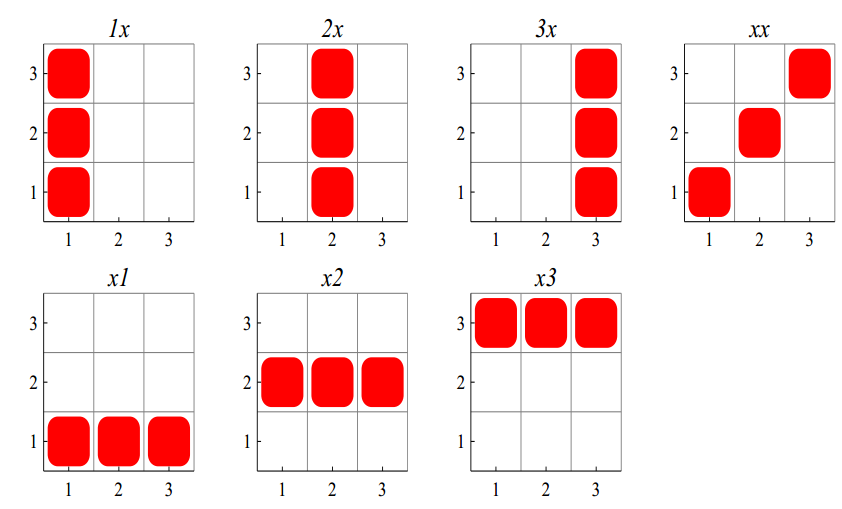
\includegraphics[scale=0.35]{cblines.png}
\caption{Combinatorial lines in $[3]^2$ (Source: \cite{polymath2010density})} \label{cl}
\end{figure}

For $k=3$ and $n=8$, a combinatorial line over alphabets $\{1,2,3\}$ for the word  $w(x)=1xx2x23x$ is the set :

$\{w(x;i)=1ii2i23i: \ i\in [3]\}=  \{11121231, 12222232, 13323233 \}.$ As matrix representation, this combinatorial line can be expressed as:

\begin{center}
$\left(\begin{array}{cccccccc}
1 & 1 & 1 & 2 & 1 & 2& 3 &1\\  1 & 2 & 2 & 2 & 2 & 2 & 3 & 2\\ 1 & 3 & 3 & 2 & 3 & 2 & 3 & 3 
\end{array}  \right)$
\end{center}

%\Jnote{This is not consistent with your previous notation.}

Sets which do not contain any combinatorial lines are called  \textit{line-free}. 

\begin{thm}[Hales-Jewett theorem]   For every pair of positive integers $k$ and $r$ there exists a positive number $HJ(k, r)$ such that for every $n \geq HJ(k, r)$ and every $r-$colouring of the set $[k]^n$ there is a
monochromatic combinatorial line.   \label{hj1} 	\end{thm}

There are several proofs of Hales-Jewett theorem. The original proof has been given by \cite{hales1987regularity}. \cite{shelah1988primitive} proved a primitive recursive\footnote{Primitive recursion is a procedure that defines the value of a function at an argument $n$ by using its value at the previous argument $n-1$.  On computer, a primitive recursive bound can be implemented only using do-loops (see https://plato.stanford.edu/entries/recursive-functions/$\#1.3$).} bound for the Hales-Jewett number using simple induction.
\cite{nilli1990shelah} presented a compact form of Shelah’s Proof of the Hales-Jewett Theorem.  This condensed form states that for every $k,r \geq 1$, $HJ(k,r) \leq \frac{1}{kr} h_4 (k+m+2)$ where  the function $h_i$ is defined as: $h_1(n)=2n$; for $i>1$, $h_i=\underbrace{h_{i-1}(h_{i-1}(\ldots h_{i-1}(1)))}_{h_{i-1} \text{ is taken } n \text{ times}} .$
\Jnote{s/$h_i$/$h_i(n)$. Also put this formula as separate equation.}

 \cite{matet2007shelah} gave a variant of Shelah’s proof of the Hales–Jewett theorem by replacing Shelah’s pigeonhole lemma by an appeal to Ramsey’s theorem.

The Hales-Jewett theorem has also a density version. By considering a nonempty subset  $A$ of the set $[k]^n$, the density of $A$ inside $[k]^n$ is a positive real number $\delta=\frac{|A|}{k^n}$. Values of $\delta$ are bounded by $0$ and $1$, that is $0< \delta \leq 1.$ 

Let denote by $DHJ(k, \delta)$ the density Hales-Jewett number. The density version of Hales-Jewett theorem is announced as follows:

\begin{thm}[Density version of Hales-Jewett theorem]   For any $k \in \mathbb{Z}^+$ and any real number $0< \delta \leq 1$,  there exists a positive integer $DHJ(k, \delta)$ such that if $n \geq DHJ(k,\delta)$ and $A$ is any subset of $[k] ^n$ with $|A| \geq \delta k^n$, then $A$ contains a combinatorial line.  \label{hj2}	\end{thm}

The proof of the density version of Hales-Jewett theorem has been demonstrated by \cite{furstenberg1991density} using ergodic methods\footnote{Ergodic theory studies dynamical systems with an invariant measure and related problems. Ergodic theory can be described as the statistical and qualitative behavior of measurable group and semigroup actions on measure spaces.}. \cite{polymath2012new} gave an elementary non-ergodic proof of the density version of Hales-Jewett theorem by giving a quantitative bound on how large $n$ needs to be and qualified this theorem as one of the fundamental results of Ramsey theorey. A simplified version of \cite{polymath2012new} has been given by \cite{dodos2013simple} using  a purely combinatorial proof of the density Hales–Jewett Theorem.

There are four important theorems we have talked about: Van der Waerden's theorem \eqref{vd1}, Szemerédi's theorem \eqref{sz1}, Hales-Jewett theorem \eqref{hj1} and density Hales-Jewett theorem \eqref{hj2}. 
In \eqref{vsz} we have shown that Szemeredi's theorem implies Van der Waerden's theorem. It is reasonable to show these three implications: the density version of Hales-Jewett theorem implies the Hales-Jewett theorem
\Jnote{Put comma here.}
Hales-Jewett theorem implies  Van der Waerden's theorem, and the density version of Hales-Jewett theorem implies Szemerédi's theorem.

\subsection{Density version of Hales-Jewett theorem implies the Hales-Jewett theorem}

To show that this density version of Hales-Jewett theorem implies the Hales-Jewett theorem, we need only to set as in  \eqref{vsz}, $\delta=\frac{1}{r}.$ By $r-$colouring the set $[k]^n$, that is by partitioning to $r$ classes,  if $A_{max}$ is the set containing the maximum number then $|A_{max}| \geq \frac{k^n}{r}=\delta k^n.$ Hence, according to \eqref{hj2}, $A_{max}$ contains a combinatorial line.

\subsection{Hales-Jewett theorem implies Van der Waerden's theorem}

To show that the Hales-Jewett theorem implies Van der Waerden's theorem, we need only to show that combinatorial line corresponds to the arithmetic progression.
%\Jnote{``combinatorial lines correspond to arithmetic progressions''.}
%\Jnote{I'm not sure what you are trying to say here.}

Let us  assume that the Hales-Jewett theorem is true and show that the combinatorial line of $k$ elements contained to the subset $A$ corresponds to the arithmetic progression of length $k$.

We have defined $[k]$ as the set $\{1,2,\ldots, k\}.$ Instead to start by $1$, let us start by $0.$ In this part, $[k]$ expresses the set $\{0,1,\ldots, k-1\}.$ It is obvious that $[k]=\mathbb{Z}/k\mathbb{Z}.$

Let $n$ be the positive number of the Hales-Jewett theorem, then the set $[k]^n=(\mathbb{Z}/k\mathbb{Z})^n=\{(y_0,y_1, \ldots, y_{n-1}): \ y_i \in [k] \}$ has $k^n$ elements. Similarly, $[k^n]=\{0,1,\ldots, k^n-1\}$ has also $k^n$ elements. Note that the set $[k^n]$ contains natural number (in base 10).
\Jnote{Just natural numbers, not in any base.}
While, elements of the set $[k]^n$ are
\Jnote{s/are/can be interpreted as}
the digits  in base$-k$ number system of the numbers $\{0,1,\ldots,k^n-1\}.$

Let us consider the bijection $f:[k]^n \longrightarrow [k^n]$ defines as follows:

$$f(y_0,y_1,\ldots, y_{n-1})=y_0+y_1k+y_2 k^2+\ldots+y_{n-1}k^{n-1}.$$

Let $w(x) \in ([k] \cup \{x\})^n\setminus [k]^n$ be an $x-tring.$ The combinatorial line generates by $w(x)$ is a set of $k$ elements defined by  $\{w(x;i):i\in [k]\}.$

Let $w(x;i)$ and $w(x;i+1)$ be two consecutive elements of the combinatorial line generates by $w(x)$. We denote  $w(x;i)=(y_{0,i},y_{1,i},\ldots, y_{n-1,i}) $ and $w(x;i+1)=(y_{0,i+1},y_{1,i+1},\ldots, y_{n-1,i+1})$ where  the elements  $y_{j,i} \in [k]$ for $0 \leq j \leq n-1$ and $0 \leq i \leq k-1.$

The difference
\Jnote{Mention that your arithmetics now is in a vector space
  (so $w(x;i)$ is a vector).}
between two consecutive elements $w(x;i)$ and $w(x;i+1)$
of this combinatorial line is a constant. Let us call this constant $l=(l_0, l_1, \ldots, l_{n-1})= w(x;i+1)-w(x;i)$.


For $j\in \{0,1,\ldots, n-1\}$, $l_j$ has two values:

$l_j= \left\lbrace \begin{array}{ll}1 & \text{ if } y_{j,i}\neq y_{j,i+1} \\ 0 & \text{ if } y_{j,i} =  y_{j,i+1}   \end{array} \right. .$
%\Jnote{$l_j=1$ or $l_j=x$?}

Let $w(x;0)=(y_{0,0},y_{1,0},\ldots, y_{n-1,0})$ be the first element of the combinatorial line generated by $w(x)$ . Then, for $0\leq i \leq k-1$ an element $w(x;i)$ of the combinatorial line can be expressed as: $$w(x;i)=w(x;o)+il.$$
\Jnote{Change o to $0$.}

Let call by $a$ the image of $w(x;0)$ by $f$, that is $a=f(w(x;0))$ and by $d$ the image of $l$ by $f$, that is $d=f(l).$ $a$ and $d$ are both integers.  We denote by $J$ the set $\{j: \ y_{j,i}\neq y_{j,i+1} \}.$ The integer $d$ can be expressed as:
$$d=f(l)=l_0+l_1k+\ldots+l_{n-1}k^{n-1}=\sum_{j=0}^{n-1}l_jk^j= \sum_{j\in J} k^j.$$
Thus, $f(w(x;i))=a+id$, $a$ and $d$ fixed, $0\leq i \leq k-1$. Hence, the set $\{a+id: \ i\in [k]\}$ forms an arithmetic progression of length $k.$ So, for any combinatorial line of $k$ elements corresponds an arithmetic progression of length $k.$

Therefore, the Hales-Jewett theorem implies Van der Waerden's theorem.
\Jnote{Your explanation so far was good, but you are not finished yet.
  You are proving VdW, so you have $k$ and $r$.
  What $k$ and $r$ do you choose for HJ (the same, but you have to say it).
  What is $N_0$ that you get for VdW in terms of $HJ(k, r)$?}

\subsection{Density version of Hales-Jewett theorem implies Szemerédi's theorem}

We have shown that any combinatorial line of $k$ elements corresponds an arithmetic progression of length $k.$ Also, we have established that there exists a bijection between $[k]^n \longrightarrow [k^n].$ So, we just need to set $N(k,\delta)=k^n$ to show that the Hales-Jewett theorem implies the Szemerédi's theorem.
\Jnote{Stil not fixed. What is $n$ here?}

As we have shown that Szemerédi's theorem implies Van der Waerden's theorem, we can establish by transitivity that the density version of Hales-Jewett implies Van der Waerden's theorem.

\subsection{Density Hales-Jewett number}

\begin{defn} Let $n \geq 0$ and $k \geq 1.$ The \textit{density Hales-Jewett number}	denoted by $d_{k,n}$ is defined as the size of the largest subset of the set $[k]^n=\{1,2, \ldots, k\}^n$ which contains no combinatorial	line. \end{defn}
If $W$ is the largest subset of $[k]^n$ without a combinatorial line, then $d_{k,n}=|W|.$ $W$ is also called a \textit{line-free}. We denote by $\Delta_{k,n}=\frac{|W|}{n^k}$ the density of $W.$

The combinatorial line is to $\Delta_{k,n}$ for the density Hales-Jewett number
\Jnote{s/number/theorem}
what the arithmetic progression is to $\delta_{k,N}$ for the Szemerédi's theorem. That is, the major  difference between $\Delta_{k,n}$ and $\delta_{k,N}$ is located on the definition of the largest subset: combinatorial line for the first and arithmetic progression for the second. 

\cite*{furstenberg1991density} showed that $d_{k,n}=o(k^n)$ (respectively $r_{k,N}=o(k^n)$) as $n\longrightarrow \infty.$
\Jnote{Rephrase: Density Hales-Jewett theorem is equivalent to saying
  that $d_{k,n} = o(k^n)$.}
Informally, the little-o means that the upper bound for $d_{k,n}$ (respectively $r_{k,N}$) but that $d_{k,n}$ (respectively $r_{k,N}$) can never be equal to $k^n.$
\Jnote{Rephrase: ...it means that $d_{k,n}$ grows slower than
  any constant fraction of $k^n$}.
In another words, the growth rate of $d_{k,n}$ (respectively $r_{k,N}$) is less
\Jnote{s/less/strictly less}
than the growth rate of $k^n.$

For $k=1$ and $k=2$, the density Hales-Jewett numbers $d_{1,n}$ and $d_{2,n}$ are trivial.
\Jnote{Don't say it is trivial for $k=2$. You are not allowed to say it is
  trivial if you cannot prove it (can you?). You can say that it is easier
  than other cases.}
That is, $d_{1,n}=1$ and $d_{2,n}= {n \choose \lfloor \frac{n}{2} \rfloor}$ where $\lfloor x \rfloor $ is the floor function defined as following: $\lfloor x \rfloor =n \Longleftrightarrow n \leq x < n+1 \Longleftrightarrow  x-1 < n \leq x .$
\Jnote{Definition of floor is not correct (you have to say $n$ is integer).
  You can delete it anyway.}

\cite{polymath2010density} used both human and computer-assisted arguments to compute some non-trivial density Hales-Jewett numbers for $k=3$ when $n= 0,\ldots,6.$

\begin{table}[h]
\centering
\begin{tabular}{|c|c|c|c|c|c|c|c|}
\hline 
$\mathbf{n}$ & 0 & 1 & 2 & 3 & 4 & 5 & 6 \\ 
\hline 
$\mathbf{d_{3,n}}$ & 1 & 2 & 6 & 18 & 52 & 150 & 450 \\ 
\hline 
\end{tabular}
\caption{Some known values of $d_{3,n}$ for $ n= 0,\ldots,6.$}
\end{table} 

Let us give examples of the line-free derived from \cite{polymath2010density} for $k=3$ and $n=2$ and $n=3.$
\begin{itemize}
\item For $n=2$, there are 4 largest line-free of $[3]^2$ each with cardinality $d_{3,2}=6 :$ $ \{12, 13, 21, 22, 31, 33 \}$, $\{11, 12, 21, 23, 32, 33 \}, \{11, 13, 22, 23, 31, 32 \}, \{12, 13, 21, 23, 31, 32 \}.$
\item For $n=3$, the largest line-free of $[3]^3$ with cardinality $d_{3,3}=18$ is: $\{112, 113, 121, 122, 131, 133, 211, 212, 221, 223, 232, 233, 311, 313, 322, 323, 331, 332 \}.$
\end{itemize}
\Jnote{Fix too long lines here.}

Knowing that $d_{3,0}=1$, $d_{3,1}=2$,  \cite{polymath2010density} gave an upper bound of $d_{3,n}$ for all $n$: $$d_{3,n+1} \leq 3 d_{3,n}.$$

\cite{polymath2010density} presented some approximations of the lower and upper bounds for general case of $d_{k,n}.$ We present these bounds in \eqref{fk} for establishing the connection between Hales-Jewett theorem and the parallel repetition of multi-prover games. This connection is developed in the end of the  chapter 3. 


 
 
 
















%The idea is to let  $ N_0=\ell^{n_0}$, and to associate with every number in $ [N]$ the digits in its expansion in the base-$ \ell$ number system. Then any combinatorial line would correspond to an arithmetic progression. (But not conversely. Why?)




 % Chapters might go from 2. problem statement, 
                 % through 3. model, to 4. analysis & results
%\input{chapter7}% Chapters might go from 2. problem statement, 
\chapter{Methodology}
This chapter presents detailed description  of the concepts underlying the techniques and tools that are employed to achieve the goal of the research. First of foremost we describe how the LDA algorithm works in gensim with respect to the how the results were obtained. All other concepts and prior tools adopted for data preprocessing are also explained.

\section{Data}
The source of the data for this research is from the website of IFRC. Practically the data was obtained by algorithms implemented in the R studio, automatically downloaded the over one thousand pdf reports from the website. Each report is named a name of a country depicting that the reports describes disaster that occurred in a particular country. Each report has an appeal id, several documents might refer to the same appeal id. The appeal id is the unique code given a particular report. Reports describing the same event have the share the same appeal id.

\section{Packages and Modules}
Before training the model on the data some modules that are important to enable smooth running of the algorithms were were imported. Apart from Gensim and NLTK that are deeply explained in subsequent sections of this chapter, the role of  the remaining are briefly highlighted below.
\begin{itemize}
\item os: This module was used to locate path of the directory containing files needed to do the machine learning. And also to combine the various paths to these files
\item codecs:Specifically codec.open from the codecs module opens  the encoded text files. It takes 5 positional arguments but 4 were necessary to obtain the required output. They are "filename", "mode=r", "encoding=utf-8" and "errors=ignore", the "bufffering' argument was ignored.
\end{itemize} 

\subsection{Gensim}
\begin{flushleft}
Gensim is an open source toolkit implemented in python to execute task involving vector space models and topic modelling \cite{rehurek2010software}. Some features of Gensim employed in this research are "term frequency inverse document frequency (TFIDF)" and "LDA", "LSA". Before executing the above features the "corpora" and "doc2bow" modules are used to represent large collection of texts and to convert the text collection into vectors respectively.
\end{flushleft}
\subsection{Natural  Language Toolkit (NLTK)}

This is also an open library with set of modules that enhances the processing of human language. It is originally developed by Steven Bird and Edward Loper both in  the Department of Computer and Information Science at the University of Pennsylvania. This provided a landmark for researchers to contribute to making it more robust and an efficient library. The "corpus" and the "tokenize" are some modules relevant in topic modelling.
\section{Data Preprocessing}
\begin{flushleft}
This section highlights the preliminary techniques applied on the data data sets before training model. Preprocessing helps to prepare the data to be compatible to the training algorithms, but also removes noise (irrelevant items) from the data, since their presence do not contribute towards obtaining desired results. This method is very important in topic modelling because it gives an idea to understanding the various terms in the corpus.
\end{flushleft}
\subsection{Tokenization}
\begin{flushleft}
This describes the process of splitting  a text or a collection of texts  into each single term constituting the text. Each term is known as the token. It can be a "word", "symbols", "punctuations", "numbers". For example given text "she won a prize worth 30 million dollars", after tokenizing we have "she", "won", "a", "prize", "worth", "30", "million", "dollars". Prior to creating a vector representation of terms in the document tokenizing is done. The Natural Language Toolkit (NLTK) library is employed to implement this process.
\end{flushleft}
\subsection{Stop Words, Punctuations  and Irrelevant Terms}
\begin{flushleft}
Prior to training the model on the data, words are commonly known as common words, such as "is", "at", "the", "or" are removed. This words are removed because mostly they do not represent the major significant terms to understanding a given article or document. Stop words are also removed to reduce the number number of unique tokens in the corpus. The nltk has a model that automatically removes stop words. Punctuations and numbers are removed, it is reasonable to mention that the former cannot contribute to uncovering the  thematic meaning of documents, they are just symbols. Because we are dealing with a number of documents and documents have pages, terms related to page numbers are removed. As well as terms with  length of one, for example "x", "y" and empty spaces are deleted. 

\end{flushleft}
\subsection{Dictionary and Corpus}
\begin{flushleft}
To be able to train a topic model, the data sets have to transformed to specific form to make sure the model is able to work with it. The dictionary is a list of unique words in all the documents. It is created with the "corpora.Dictionary" module from gensim tool kit. Having a dictionary created allows us to know the total number of unique terms and all words positions in all the documents collections.
\end{flushleft}
A corpus represents the converted words to bag of words, each word is in a tuple form , the first and second component stands for the  "word id" and its  "frequency" respectively in a particular document. For example $(1452,100)$ in document 1 means the $1452th$ word appears 100 times in document 1.
\section{Term Frequency Inverse Document Frequency (TFID)}
\begin{flushleft}
This measures the extent to which words are important in a document. In topic modelling we want to find a group of words that describes a vocabulary. For example topic modelling a document that talks about a university, words such as "classrooms", "library", "lecturs", "Courses", "Grades" would tend to be the most important words that describe the topic. It is worth noting that important words are not necessarily the most frequent words, possible to be judged by our intuitive notions. 
\end{flushleft}

\begin{flushleft}
The TFIDF transforms a vector of integer values into a vector of real values, maintaining the dimension of the original vector.After transformation  features which are not frequent in the corpus may have their values increased. That does not mean that  all rare words important, some may not be significant at all in the description of the topic.
%\Jnote{Rare words all rare words?}
For instance dealing with our "university" document, a word like "congregation" may rare but then it is significant towards describing the vocabulary. On the other hand a word such as "consequently" may appear very frequent which in this case does not really say anything about the topic. The most frequent words are
most words such as “the” or “and,” which helps to construct a sentence, thereby making it readable and understandable.These words do not carry any importance to help topic model a document.They are stop words and they are removed before the modelling irrespective of their number.
\end{flushleft}
 Given a collection of document with each document $d$ containing words, where each word in the document is denoted $i$. The frequency of occurrence of a word $i$ in document $d$ is denoted $f_{id}$. The term frequency $TF_{id}$ computed as:
 
$$TF_{id}=\frac{f_{id}}{\text{max}_tf_{td}}$$.
%\Jnote{What is $j$?}
Which means that the  frequency of the word  i in document d is $f_{id }$normalized by dividing
it by the term with the highest frequency in the same document of occurrence with stop words exclusive.
%\Jnote{You forgot math mode.}
Intuitively the word which occurs most frequently would have  would have a $TF$ of 1,
%\Jnote{word which occurs what?}
and other words get fractions as their term frequency for this document.
The IDF for a word $i$ which occurs in $d$ of the $D$ documents is computed as:
$$IDF_i=log_2\frac{D}{d_1}\text{.}$$
The TFIDF for a term $i$ in document $d$ is will now be:
$$\text{TFIDF}=TF_{id}\cdot IDF_i \text{.}$$
\section{LDA Implementation}
This model is a type of topic model that is based on the imaginary  assumption that 'words are used to generate documents' or simply "it is a document generative process".
For example given $N$ words for a particular document. To generate the documents given the words,firstly choose words deemed to be abstracts topics of  the entire corpus, where each topic has a probability  value $ \theta_d $, known as the per document topic proportion. For each word  we choose a topic $ Z_{d,n} $, from the list of topics already chosen. And then choose a word $ W_{d,n} $ from that topic . Each word chosen is placed in the document and the process is repeated until all the $ N $ words are exhausted to fill the document. The only variable that is observed is the $ W_{d,n} $, the remaining are hidden variables.


In practical terms the LDA model works in a reversed manner. What it actually does is that it finds the latent variables given the $ W_{d,n} $, using the posterior distribution. Because the posterior is difficult to compute the variational inference approximates the posterior. This approximation are embedded in the LDA algorithm. The LDA model in gensim takes several positional arguments but only seven is used, their functions in the model are briefly described below.
\begin{itemize}
\item Corpus: This is the vectorized form of all the documents. Each list of tuples represents a document. 
\item Id2word: Instead of the model using the word numeric id's in the corpus, it is assigned a dictionary containing the words. This makes it easier to read the model output because words constituting a topic will be displayed. Without assigning the id2word the dictionary the words which are distribution over a topic will be shown as numeric id's. 
\item Num\_topics: This takes the number of topics that the model should output. The number of topics chosen is subjective and could be subjected to the number of documents in the corpus. 
\item Chunk\_size: Depending on the number of documents that the model  should process at a time is assigned to this parameter.The choice of documents to be processed is dependent on the total number of documents in the corpus. It our model the 1259 is processed at once.
\item Update\_size: This tells the model how many times to update per the given chunk\_size. The default size in the model is 1 which was maintained.
\item Passes: Is the number of times that the corpus should be passed over in the modelling process. High value of passes is recommended to obtain better results.
\item Alpha: The alpha is a hyper parameter value responsible for controlling the per document topic distribution from the Dirichlet distribution. The "alpha"parameter can be assigned to any arbitrary value, but in our case it assigned to "auto" to allow the model to learn the data and properly assigned an alpha parameter value. Higher alpha values produce more topics, and thus makes documents looks more similar to each other, and for low alpha values, results in  documents having few topics. 

\cite{griffiths2004finding} Suggested an alpha ($\alpha$) value of $\frac{50}{T}$, where $T$ is the number of topics and 0.1 for eta ($\eta$).
\end{itemize}

\section{Visualizing the Topic Model}
Visualizing topic models is very important because it gives a
a clear graphical representation of the topics and their associated  terms. One  tool that is used to visualize topic models is the LDAvis. After the LDA model is fitted, the LDAvis is used to interpret the model and understand it better. It takes the "corpus", "Dictionary" and the "LDA model" to produce a visual results. The following can be determined with the LDAvis tool.
\begin{itemize}
\item Proportions of each word in a topic and in the entire corpus.
\item How often Topics that occur in the topic model.
\item The relationship between topics in the topic model.
\end{itemize}

\section{Python and R}
The research employs the Python and R programming languages to implement all the task necessary to achieve the desired goal associated with this research. Preliminary the R studio provided an environment to execute algorithms that scrapped the pdf reports from the IFRC website. Converting these reports from pdf to txt formats were also handled by the R studio. 
All other algorithms pertaining to the machine learning process were done in python.
%Theorems before the chapter's first section will be dot-zero, 
%and their numbering is completely wrong. You can avoid this
%by simply always starting a chapter with a section. Ta Da! 
%It will probably help you structure your essay anyway. 
%
%\begin{thm}[My Theorem2]
%This is my theorem2.
%\end{thm}
%\begin{proof}
%And it has no proof2.
%\end{proof}
%
%\section{See?}
%
%Text text text text text text text text text text text text text text
%text text text text text text text text text text text text text text
%text text text text text text text text text text text text text text
%text text text text text text text text text text text text text text
%text text text text text.
%
%\begin{thm}[My Theorem2]
%This is my theorem2.
%\end{thm}
%\begin{proof}
%And it has no proof2.
%\end{proof}
%
%Text text text text text text text text text text text text text text
%text text text text text text text text text text text text text text
%text text text text text text text text text text text text text text
%text text text text text text text text text text text text text text
%text text text text text.
%
%\begin{align} % do not use eqnarray. 
%\label{2ya}
%x & = y + y\\
%\label{2yb}
%& = 2y
%\end{align}
%see equations \eqref{2ya} and \ref{2yb}
%
%\section{More}
%
%Here's a conjecture
%\begin{conj}
%The washing operation has fixed points.
%\end{conj}
%
%and here's an example
%
%\begin{exa}
%100 FRW coin.
%\end{exa}
%
%\subsection{This is a subsection}
%
%\section{This is a section}
 % You do not need to have exactly 4 chapters.
                 % It is probably a good minimum, with 5 chapters 
                 % average, and 7 chapters might be a maximum.
\chapter{Compartmental and Stochastic Models}
\section{Deterministic Models}

\subsection{SIR Model}

In the SIR model the population is partitioned into three compartments susceptible, infected and recovered This is the basis for most epidemiological models \citep{m1925applications}. In building the model the number of individuals susceptible, infected and recovered is assumed to be differentiable over time.
The simple epidemic model is given by,
\begin{center}
\begin{align} \label{eqn4.1}
\frac{dS}{dt} &= -\beta SI,\\
 \frac{dI}{dt} &=\beta S I - \gamma  I, \\
 \frac{dR}{dt} &= \gamma  I.
\end{align}
\end{center}

$N = S + I + R.$
The model is based on the assumption that susceptible individuals become infected at a rate $\beta$ proportional to the number of people infected and susceptible at time $t$ and infected people recover at $\gamma$ rate. The reciprocal $\frac{1}{\gamma}$ is referred to as the average infectious period. Another assumption in this model is that the population remains constant, thus it does not take int account the demographic changes of the population. Figure \ref{fig 4.1} shows the compartmental diagram for an SIR model without demographic dynamics.
\begin{figure}[h!]
\centering
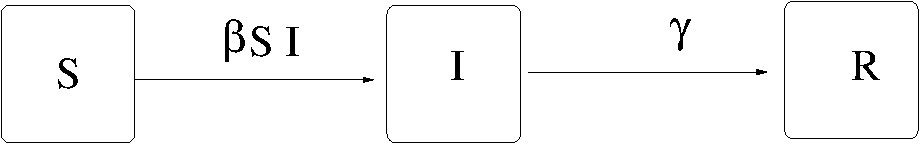
\includegraphics[scale=0.5]{images/sir.jpg} 
\caption{SIR compartmental diagram}\label{fig 4.1}
\end{figure}



\subsection{Model Analysis}
We determine the equilibrium and the stability of \ref{eqn4.1}, but since $N =S + I + R$ knowing $S$ and $I$ implies that we can solve for  $R$. Hence our system of equations can be reduced to 
\begin{align}
\frac{dS}{dt} &=-\beta SI. \label{eqn4.11} \\
 \frac{dI}{dt} &= \beta S I - \gamma  I \label{eqn4.22}.
\end{align}
 With $S(0) >0$, $I(0) > 0$ and $R(0) =0$ as the initial conditions for the model.
 We now calculate the disease free equilibrium and endemic equilibrium by equating equations \ref{eqn4.11} and \ref{eqn4.22} to zero then solving them. Despite its extreme simplicity, this model equation \ref{eqn4.1} cannot be solved explicitly. That is, we cannot obtain an exact analytical expression for the dynamics of S and I
though time, instead the model has to be solved numerically.

The equation \ref{eqn4.11} gives two import insights in understanding the spread of disease and has since been used in infectious disease modelling for a long time.

\subsection{Threshold Phenomenon} 
It is important to determine whether the infection will result in an epidemic or not and what are the determining factors. Consider the initial stage after $I (0) $ individuals have been infected in a population with $S (0) $ susceptible. Equation \ref{eqn4.22} can be rewritten as,
\begin{equation} 
\frac{dI}{dt} = I \left(\beta S -\gamma \right)\label{4.14}
\end{equation}
In equation \ref{4.14} if the initial susceptible (S(0)) is less than $\frac{\gamma}{\beta}$, then $\frac{dI}{dt} < 0 $. This means that there will be no epidemic in this case.

This result was coined by \cite{m1925applications} and  is refereed to as the threshold phenomenon. The initial S(0) must exceed the threshold $\frac{\gamma}{\beta}$ for an epidemic occur. In  other words the relative removal rate $\frac{\gamma}{\beta}$ must be small enough to allow the occurrence  of the epidemic.
 
 The reciprocal of the of relative removal rate is called the basic reproductive ratio and is one of the most important quantities in epidemiology. The basic reproduction ratio is defined as the average number of secondary cases arising from an average primary case in an entirely susceptible population. It measures measures the maximum reproductive potential for an infection. For the our SIR model in equation \ref{eqn4.1} it is given by:

\begin{equation}
R_0 = \frac{\beta}{\gamma}\label{eqn 4.15}
\end{equation}
 
For initial susceptible $S(0) = 1$, if $R_0 >1$ then there will be an outbreak and if $R_0<1$ the will be no outbreak. It can be noted that every disease has a different $R_0 $ value and also depending on the population's contact pattern the $R_0$ value will differ.

 \subsection{Epidemic Burnout}
 The threshold phenomena gives a description of what happens in the initial stages after introduction of an infection. Another important quantity we get from the SIR model is the long term state of the infection. From they system in equation \ref{eqn4.1} we take
 
 \begin{align}
 \frac{dS}{dt} &= -\beta S I \label{4.16}
 \\ \frac{dR}{dt}& = \gamma I \label{4.17}
\intertext{  dividing  equation \ref{4.14} by equation \ref{4.17} we get } \nonumber
\\ \frac{dS}{dR}& = \frac{-\beta S}{\gamma}
= - R_0 S \label{4.19}
 \end{align}
 Integrating equation \ref{4.19} with respect to R, we get; 
 
 \begin{align}
 \int{\dfrac{dS}{S}} &= -\int{ R_o dR}
 \\ ln S &= -R_0 R + k
 \\ e^{ln S} &= e^{-R_0 R + k}
 \\  S(t) &= e^{-R_0 R(t)} e^{k}
 \intertext {assuming R(0) = 0} \nonumber
 \\ S(t) = S(0)e^{-R_0 R(t)} \label{eqn 4.1.13}
 \end{align}
 
 Hence, as the epidemic develops, the number of susceptibles reduce. The numbered of recovered does not start increasing immediately because of infectious period, but eventually it does. Their number of susceptibility in the population will always be above zero as can be seen in equation \ref{eqn 4.1.13}.
 
From equation \ref{eqn 4.1.13}, $s(t) \geq e^{-R_o}$ since $R(t) <1$. Thus, there will always be a proportion of susceptibles in the population.  The epidemic burnout gives the intuitive idea that the chain of transmission eventually breaks due to the decline in infectives not due to lack of susceptibles \citep{haran2009introduction}.
 
 \subsection{Disease free equilibrium}Adding demographic parameters to \ref{eqn4.1} we get a new system of equations. That is, adding a parameter for birth rate and death rate, hence the population is no longer closed in this case.
 
 \begin{align}
 \dfrac{dS}{dt}& = \mu - \beta S I - \mu S \label{1}
 \\ \dfrac{dI}{dt}&= \beta SI - \gamma I -\mu I  \label{2}
 \\ \dfrac{dR}{dt} &= \gamma I - \mu R \label{3}
 \end{align}
 
 Using the same procedure we used to get the equation \ref{eqn 4.15} it can be shown that the $R_0$ for this model is \begin{equation}
R_0 = \frac{\beta}{\mu + \gamma} \label{eqn 4.2.17}
\end{equation}
 
 Now we calculate the equilibria  of the model by setting  equation \ref{1}, \ref{2} and \ref{3} to zero, that is $\dfrac{dS}{dt}= \dfrac{dI}{dt}= \dfrac{dR}{dt}= 0$ and denote by $S^*, I^*$ and $R^*$  values of  S, I and R that satisfy this condition. 
 From equation \ref{1} we get
 \begin{align}
  \mu -\beta SI - \mu S = 0 
  \\ \mu - S (\beta I + \mu ) = 0
  \\ S = \dfrac{\mu}{\beta I + \mu}
  \end{align}
 It can be shown that $S^* I^* R^* = (1,0,0)$ is the epidemic free equilibrium.
 
  To establish the endemic equilibrium , we factorize $I$ in  equation \ref{2} and  we get,
 \begin{align}
I (\beta S -(\gamma+ \mu)) = 0
 \intertext {thus we get}
 I = 0 \rightarrow S = \frac{\gamma+ \mu}{\beta}
 \end{align}
 Therefore, $I^* = 0$ and $S^* = \frac{\gamma+ \mu}{\beta}$, but since $I^* = 0$ is a disease free equilibrium. We concentrate on $S^* = \frac{\gamma + \mu}{ \beta} = \frac{1}{R_0} $ see \ref{eqn 4.2.17}
 
 Now, we take $I \neq  0 $ and solve \eqref{3}. Since $S+R+I =1$
 \begin{align}
 \gamma I - \mu (1 -S -I) = 0
 \\ \gamma I - \mu I -\mu (1-S) = 0
 \\ I = \frac{\mu}{\beta} R_0 \left( 1- \frac{1}{R_0} \right)
 \\ I = \dfrac{\mu}{\beta} (R_0 -1) 
 \end{align}
 
 Thus the endemic equilibrium point $( S^*,I^*,R^*)$ is 
 $\left( \frac{1}{R_0}, \frac{\mu}{\beta} (R_0 -1), 1 -  \frac{1}{R_0} \frac{\mu}{\beta} (R_0 -1) - \frac{1}{R_0} \right)$
 
 
  \subsection{Stability of the Model}
 Once an outbreak occurs, its important to understand the long term behaviour of the outbreak and finding the stability of the model gives an insight on this. In other words, calculating the stability of the model is establishing at which point the epidemic burn out will occur.
 \subsection{SEIR Model}
The susceptible, exposed, infected and recovered models add a new comportment to the previously discussed SIR Model. The earlier models assume that once a person is infected, they become infectious immediately. In this model an assumption is made that once a person is infected there is an intermediate stage between the time of infection and when they become infectious, this may be refereed to as the latent or incubation period of the infection. The system of equations will be;

\begin{align}
S'& = \mu -\beta S I - \mu S \label{5} \\
E' &= \beta S I - (\mu + \gamma) E  \label{6}\\
I' &= \gamma E - (\alpha + \mu I) \label{7}\\
R' &= \alpha I  - \mu R \label{8}
\end{align}
where $\beta$ is the rate at which susceptible individuals become infectious, $\gamma$ the rate at which infected individual become infection. The quantity $\frac{1}{\gamma}$ is called the latent period of the  infection and$\alpha$ is the recovery rate.
In this model the total number of infected individuals is given by $E +I$ and  we assume that our system is density dependant thus $S + E + I + R = 1$ and  that the population is constant implying that the birth rate ($\mu$)  = death rate $(\mu)$. Figure \ref{fig 4.2} shows the compartmental diagram of an SEIR model.
\begin{figure}[h!]
 
 \centering
 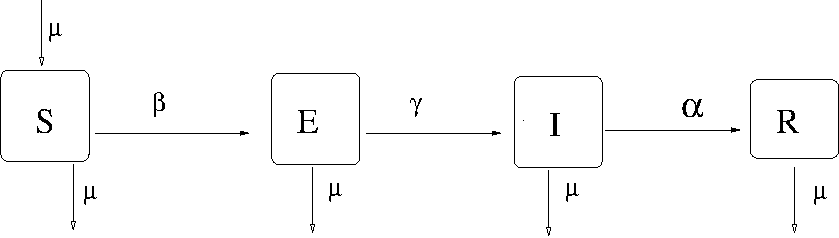
\includegraphics[scale=0.5]{images/seir.png}\label{fig 4.2}
 \caption{SEIR compartmental diagram}
 \end{figure}
  
 
Since $R = 1- S - E - I$
we can be drop equation \ref{8} from the system and  calculate equilibrium point by equating equations \ref{5} to \ref{7} to zero and solving the system of equations.

From equation \eqref{5} we get
$S = \dfrac{\mu}{\beta I - \mu}$ and from equation \ref{7} we get $I = \frac{\gamma E}{ (\alpha + \mu)}$ and from equation \ref{7} we get $ E = \dfrac{ \beta S I}{(\mu + \gamma)}$. Thus, for I = 0, E =0 and S = 1 hence, the disease free equilibrium of the system $S^*, E^*, I^* = (1,0,0)$.

 When $I^* \neq 0$ we find the disease pandemic equilibrium, which is given by
\begin{equation*}
S^*, E^*, I^*  = \left(\frac{(\alpha + \mu)(\gamma + \mu)}{\beta \gamma} , \frac{\alpha + \mu }{ \gamma} I^*, \frac{\mu}{\beta S*} \frac{\mu}{\beta} \right).
\end{equation*}

The reproductive number $R_0$  will be calculated using the new generation matrix method. Let F and V be non negative matrices,
\begin{equation}
F = \left[ \frac{\partial F_i (x^*)}{\partial j}\right]
\end{equation}  Where  $F_i (x^*)$ are the rates of new infections in compartment $i$ and 
\begin{equation}
 V = \left[\dfrac{\partial V_i(x*}{\partial j} \right]
\end{equation}
  Where $V_i (x^*)$ are the rates of transfer of infection from one compartment to another \citep{van2002reproduction}.
  $F =\left(\begin{array}{cc} 
0&0 \\ \beta&0
\end{array} \right)$ and $V = \left(\begin{array}{cc} \gamma + \mu & \gamma \\ 0& \alpha + \mu \end{array} \right)$


Therefore,
\begin{equation}\label{4.2.29}
FV^{-1} = \left(\begin{array}{cc} 
0&0 \\ \beta&0
\end{array} \right) \left(\begin{array}{cc}
\frac{1}{(\gamma + \mu)}&  \frac{-\gamma}{(\alpha +\mu)+ (\gamma + \mu)}\\ 0& \frac{1}{\alpha + \mu}  

\end{array} \right) = \left(\begin{array}{cc} 0&0 \\
\frac{\beta}{(\gamma + \mu)} &\frac{- \beta\gamma}{(\alpha +\mu)+ (\gamma + \mu)} 
\end{array}\right)
\end{equation}

The equation \ref{4.2.29} has eigenvalue values $\lambda_1$ , $\lambda_2$ as 0 and $\frac{- \beta\gamma}{(\alpha +\mu)+ (\gamma + \mu)}$ respectively.
 \begin{equation}
 R_0 = max {|\lambda_1| |\lambda_2|}
 \end{equation}
Thus the $R_0$ for the system will be $\frac{ \beta\gamma}{(\alpha +\mu)+ (\gamma + \mu)}$.

For the disease free equilibrium (1,0,0)is asymptotically stable if $R_0 < 1$ and unstable if $R_0 > 1$ \citep{van2002reproduction}. That is the solutions of the systems of equations \ref{5} \ref{7} move towards the disease free equilibrium when $R_0 < 1$.


%We examine the  behaviour of the stationary points by checking for their stability , we check the stability  of the system \ref{eqn 4.2.28}.
%
%
%
%Epidemiology compartmental models have been used for to model Infectious Diseases. Zika Virus can also be modelled using these compartmental models. A system of differential equations is used to model the dynamics of disease transmission.
%
%Zika Virus can be modelled by Susceptible , Exposed, Infectious and Recovered SEIR Model. Zika is mainly transferred by a vector(Mosquitoes). Thu the SEIR model takes into account the dynamics of pathogen transmission through vector.
%
%The compartment in this model are ; Susceptible denoted by $S_h(t)$ which is the number of people not carrying the pathogen but are prone to. Exposed denoted $E_h(t)$ This a number of people that have been exposed or have the pathogen but are not infectious. These include people that have had sex with a Zika infected person or people bitten by an infected mosquito but are yet to to exhibit symptoms and become infectious. Infectious denoted by $I_h(t)$ this compartment  comprises, people who are infected and infectious.That is they can transmit the disease to other people and they may or may not exhibit symptoms of being infected. Recovered denoted as $R_h(t)$, this compartment comprises of people that recover from the infectious or those that die or removed from the population. When some an infectious person is no longer infectious then then they are considered as recovered.
%
%Zika various is modelled with an SEIR model because one a person recovers from the infectious, studies have shown that they cannot be any reinfections. This was tested on monkeys who were cured of the infectious and Humans who have recovered from infectio\section{ Model Assumptions}
%
%
%
%The demographic variation in the number of people are not considered  and we also assume that the population among mosquitoes remains constant. This means the model does not take into death and birth among human beings. For the vectors death is assumed to be equal to birth hence the constant population. 
%
%All mosquitoes are assumed to be old to be adult mosquitoes, thus birth implies that an adult mosquito is added to into the proportion of mosquitoes.
%
%All humans have the the same probability of being infected. Either by mosquito bite or other means of  transmission. The period an organism (human or mosquito) stays in the Exposed compartment is called latent period and will be referred to as the incubation period.
%
%To model Zika virus on a random network, We take every person in the population as a vertex and when ever there is contact expected to result in the transmission of the  infection an edge is drown between the vertices. Therefore as property of a random graph, we assume that there is an equal probability of transmission between any given vertices in the graph. That is between any people in the population there is equal chance of disease transmission. This probability is used as the disease transmission rate in the SEIR model for Zika.
%
%\section{Compartmental Model}
%
%
%\section{Mathematical Model}%n \citep{posen2016epidemiology}.
%
%The vector ( Mosquitoes) also have a similar transmission of the pathogen. Though for the vector there are only three compartments. Susceptible denoted as $S_v$, this compartment comprises of a proportion of vectors that do not carry the pathogen hence can not infect anyone. The second compartment is the $E_V$ , which is a proportion of vectors that carry the pathogen but cannot infect or transmit to a human being. Lastly Infectious $I_v$ this is the proportion of vectors that can transmit the pathogens. It can be noted that since $S_v$,$E_v$ and $I_v$ are proportions, $ 0 \le S_v,E_v , I_v \le 1$ 
%

%
%The dynamical system of the transmission of Zika virus, is represented mathematically by the equations below.
%\begin{align}
%\begin{array}{lcl}  S'_h & = -&\beta_h S_h I_v  \\ E'_h & = & \beta_h S_h I_v - \alpha_h E_h  
%\\ I'_h &= &\alpha_h E_h - \gamma I_h 
%\\ R'_h &=& \gamma I_h 
%\\ 
%S'_v &=& \delta -\beta_v S_v \frac{I_h}{N} - \delta S_v
%\\ E'_v & = & \beta_v S_v \frac{I_h}{N} - (\delta + \alpha_v) E_v
%\\ I'_v & = &\alpha_v E_v - \delta I_V
% \end{array}
%\end{align}
%where :
%
%$\beta_h$  - Is the rate at which susceptible humans leave the susceptible compartment.
%
%$\alpha_h$ -  Is the rate at which exposed people become infectious.
%
%$\gamma$ - This is i the rate at which infectious individuals recover or get removed.
%
%$\delta$ -This is the birth rate of mosquitoes.
%
%$\alpha_v$ - This is the rate at which infected mosquitoes become infectious.
%
\section{Stochastic Models}
\subsection{ Stochastic SIR Model}
We will only consider an SIR model for the stochastic models. The total population $N(t) = S(t)  + I(t) + R(t)$ just as in deterministic models. Where 
\begin{align}
S(t), I(t), R(t) \in \left\lbrace 0,1,2,\dots , N \right\rbrace 
\end{align}
and $t \in \left\lbrace 0,\Delta t ,2 \Delta t, \dots \right\rbrace$. There are two independent discrete random variables  S, E and I because $R(t) = N(t) -S(t) -I(t)$. Therefore the stochastic process for the SIR model is a bivariate process $\left\lbrace S(t), I(t) \right \rbrace^{\inf}_{t =0}$ ha has a joint probability 

\begin{equation}
p_{(s+k,i+j),(s,i)}(\Delta t )= \Pr \left\lbrace( \Delta S ,\Delta I) = (k,j)\mid (S(t), I(t)) = (s,i) \right\rbrace
\end{equation}
where $\Delta S = S(t + \Delta t) - S(t)$. Hence the transition probability of the SIR model is a follows;
\begin{align}
p_{(s+k,i+j),(s,i)}(\Delta t )= \left\lbrace \begin{array}{ll}
 \beta i s / N \Delta t & (k,j) = (-1,1)
 \\ \gamma i \Delta t, & (k,j) = (0,-1)
 \\ b (N- s -i)\Delta t & (k,j) = (1,-1)
 \\ 1 - \beta i s/N \Delta t - \left[\gamma i +b(N-s) \right]n\Delta t ,& (k,j) =(0,0)
 \\ 0, otherwise
 \end{array} \right.
\end{align}
The time step $\Delta t$t must be chosen small enough such that each transition probabilities lie in the interval [0,1]. Applying the Markov property, the difference equation satisfied by the probability $p_{(s,i)} (t +\Delta t)$ can be expressed in terms of the transition probabilities.
\begin{align*}
p_{(s,i)} (t + \Delta t) &= p_{(s+1, i-1)}(t) (t) +\Delta t)rac{\beta}{N}(i -1)(s +1) \Delta t + p _{(s,i+1)} (t) \gamma (i +1) \Delta t \\ &+ p_{(s-1,i+1)}(t) b(i+1) \Delta t + p_{(s-1,i)}(t)b(N-s+1- i) \Delta t  \\&
+  {p_(s,i)}(t) \left(1 - \left[\dfrac{\beta}{N} is + \gamma i + b(N-s) \right] \Delta t\right)
\end{align*}

The difference equations can be written as in matrix form as 
\begin{equation*}
p_{(s,i)}(t + \Delta t) = P (\Delta t)p(t),
\end{equation*}
where $P(\Delta t)$ is the transition matrix and $p(t)$ is the probability distribution vector for the stochastic process.The state set is divided into two classes; the current and the transient.(N,0) is an adsorbing recurrent state while all other states are transient. The probability of an out break is given given as $1- \frac{1}{R_0}$ when $R_0 >1$ \citep{Brauer2017}.

One the main aspects in which deterministic and stochastic models differ is extinction. In deterministic SIR model an epidemic never goes to extinction in a limited time frame  because the number of infectives declines exponentially and only reaches zero at infinity.  In a deterministic framework an epidemic is said to go into extinction if it has a negative growth rate. Where as in the stochastic SIR model an epidemic is the  epidemic becomes extinct in a more direct sense, the number of infects can go to zero without waiting forever. % Conclusion is usually a chapter itself. 
%\chapter{ Spread of Zika virus on a small world network }

\begin{figure}[h!]
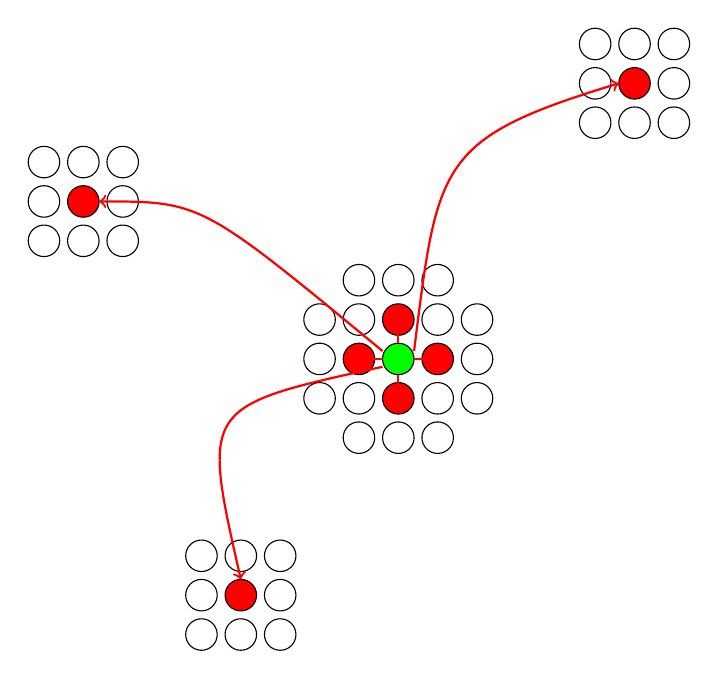
\begin{tikzpicture}
\draw (-2,5.5) circle (0.2cm);
\draw (-2,5.0) circle (0.2cm);
\draw (-2,4.5) circle (0.2cm);
\draw (-1.5,5.5) circle (0.2cm);
\filldraw[fill=red!, draw=black] (-1.5,5.0) circle (0.2cm);
\draw (-1.5,4.5) circle (0.2cm);
\draw (-1,5.5) circle (0.2cm);
\draw (-1,5.0) circle (0.2cm);
\draw (-1,4.5) circle (0.2cm);
\draw (2,2) circle (0.2cm);
\filldraw[fill=red!, draw=black](2,3) circle(0.2 cm);
\draw (2.5,2) circle (0.2cm);
\filldraw[fill =green, draw =black](2.5,3) circle(0.2 cm);
\draw (2,2.5) circle (0.2cm);
\draw(2,3.5) circle(0.2 cm);
\filldraw[fill=red!, draw=black] (2.5,2.5) circle (0.2cm);
\filldraw[fill=red!, draw=black](2.5,3.5) circle(0.2 cm);
\draw (3,2) circle (0.2cm);
\filldraw[fill=red!, draw=black](3,3) circle(0.2 cm);
\draw (3,2.5) circle (0.2cm);
\draw(3,3.5) circle(0.2 cm);
\draw(1.5,2.5) circle (0.2cm);
\draw(1.5,3) circle (0.2cm);
\draw(1.5,3.5) circle(0.2cm);
\draw(2,4) circle(0.2cm);
\draw(3.5,2.5) circle (0.2cm);
\draw (3.5,3) circle (0.2cm);
\draw(3.5,3.5) circle (0.2cm);
\draw(2.5,4) circle(0.2 cm);
\draw(3,4) circle(0.2 cm);

\draw(0,0.5) circle (0.2cm);
\draw (0,0.0) circle (0.2cm);
\draw (0,-0.5) circle (0.2cm);
\draw (0.5,0.5) circle (0.2cm);
\filldraw[fill=red!, draw=black](0.5,0) circle (0.2cm);
\draw (0.5,-0.5) circle (0.2cm);
\draw (1,0.5) circle (0.2cm);
\draw (1,0) circle (0.2cm);
\draw (1,-0.5) circle (0.2cm);


\draw (5,6) circle (0.2cm);
\draw (5,6.5) circle (0.2cm);
\draw (5,7) circle (0.2cm);
\draw (5.5,6) circle (0.2cm);
\filldraw[fill=red!, draw=black](5.5,6.5) circle (0.2cm);
\draw (5.5,7) circle (0.2cm);
\draw (6,6) circle (0.2cm);
\draw (6,6.5) circle (0.2cm);
\draw (6,7) circle (0.2cm);

\draw[red!,thick] (2,3) --(2.3,3);
\draw[red!,thick] (3,3) --(2.7,3);
\draw[red!,thick] (2.5,3.5) --(2.5,3.2);
\draw[red!, thick] (2.5,2.5) --(2.5,2.8);

\draw[draw=red!,
preaction={->,thick,draw =red!}
] (2.7,3.1) ..controls(3,5.5) and (3,5.8) ..(5.3,6.5);
\draw[ draw =red!,thick, ->] (2.3,3.1) .. controls (0,5) and (0,5) ..(-1.3,5);

\draw [draw =red , thick, ->] (2.3,2.9).. controls (0,2.4) .. (0.5,0.2);
\end{tikzpicture}
\caption{Smallworld network structure} \label{fig 5.1}
\end{figure}
The deterministic models discussed in the chapters above assume that all individuals have an equally small probability of being infected. In this section we build a model for the propagation of Zika virus based on a small world network.

Traditional models of infectious disease dynamics have a long successful history of describing and modelling infectious disease spread of many disease. They are quiet simple and tractable \citep{fu2013propagation}.

They are certain specific and common situations when the structure of social connectivity is at least as important as the infectivity of the underlying infectious agents for the study of transmission of infection and control. This is one is among the major  reasons that has motived the modelling of infectious diseases on social networks \cite{fu2013propagation}.

 We suppose that that the population is arrange in a regular grid.  Where each vertex  can infect its 4 near neighbours and a couple distant neighbours. Near neighbours in this case refers to individuals that one spends most of their time could be colleagues at work or school, people in the same house and distant neighbours refers to random individuals that one is likely to transmit the infection to. 
 
 Transmission of Zika virus is mainly through mosquito bite, thus in modelling the spread its spread on a small world network the dynamics of transmission through mosquitoes is represented by edges of the graph. An edge is drawn when there between two  vertices, whenever there is a likelihood of transmission from one to another via mosquito bite.
 \newpage
 \begin{figure}[h!]
 \centering
 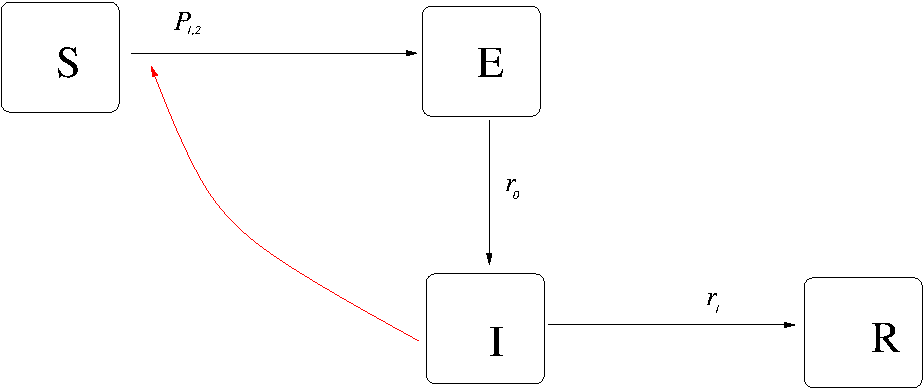
\includegraphics[scale=0.4]{images/swseir.png}
 \caption{State transition diagram} \label{fig 5.2}
 \end{figure}
 
 
 
Figure  \ref{fig 5.1}  shows the arrangement of nodes in a small world network and  figure \ref{fig 5.2} show the transmission state diagram: S to E based on the small world network network structure and the infection probabilities $p_{1,2}$: E to I with probability $r_0$ and I to R with probability $r_1$. in figure \ref{fig 5.1}, the infected green node may infect its four red near neighbours with probability $p_1$ and its three remote neighbours with probability $p_2$. By infection we mean transition from Susceptible to exposed state.

Let $p_1$ be the probability of an infected individual causing their susceptible near neighbours to become infected and $p_2$ the probability of their distant or remote neighbours to be come infected. Exposed people become infectious with probability $r_0$ and recover or get removed with probability $r_1$. In addition $n_1$ and $n_2$ is number of close neighbours and near neighbours respectively.

The number of distant neighbours $n_2$ if fixed and random for each node. That is for node i there are $n_2^{(i)} $ distant neighbours. $n_2^{(i)} $ is chosen to follow a discrete exponentially decaying distribution 
\begin{equation}
f_c(x) = \dfrac{1}{c} e^{\dfrac{-x}{\mu}}
\end{equation}
with  parameter $\mu$ proportional to the expected number of links to remote nodes and $c = \frac{1}{1- e^{frac{-1}{\mu}}}$ ensures that $f_c$ is a probability distribution function \citep{fu2013propagation}. The degree distribution in most social networks are exponentially distributed because of the celebrity effect \citep{estrada2015first}. In social networks there are few people who are with high connections and many with an average number of connections. In modelling infectious diseases these individuals are referred to as supper spreaders.

The transition probability $r_0$, the number of days an individuals is in the exposed state is as a result of bernoulli trials with mean $\frac{1}{r_0}$, follows a geometric distribution $f_X(x) = (1-p)^{x-1}p$. Similarly the infectious period follows a geometric distribution with mean $\dfrac{1}{r_o}$ \citep{fu2013propagation}.

\section{Model}
The model has seven parameters, the are $N, p_1,p_2, n_1, n_2,r_0$ and $r_1$. We let $N$ be the population size of a city or  country and is arranged in a regular grid  of side length $l $ such that $l^2 = N$. The rest of the parameters have been described above.

A  thorough review of literature in \cite{lessler2016times} indicates that $95 \%$ of patients begin to exhibit symptoms of Zika infection after $11.2$ days of infection with a $95 \%$ confidence interval of $7.6 -18$. Further the center for disease control and prevention (CDC) indicate that the incubation period for Zika virus ranges for 3 day to 14 days from infection \citep{krow2017estimated}. Therefore we estimate $r_o$  with $\frac{1}{11.2}$

$95\%$ of the cases will still have detectable virus infectiousness 18.9 days after infection with a confidence interval of 13.6 -79.4  \citep{lessler2016times}.The infectiousness in Zika infection ends 1.5 - 2 days before the virus becomes undetectable \citep{funk2016comparative}. Thus the chosen value for infectious period id $18.9 - 1.5 = 17.4$ days. Therefore $r_1$ is estimated  to be $\frac{1}{17.4}$.

Hence we have $n_1$, $\mu$, $p_1$ and $p_2$ free parameters. Without control the average number of secondary infection for Zika virus is between 3 and 6, therefore we choose 4.5 as the $R_0$. Since the number of remote neighbours is random and fixed for each, we estimate $E (n^{(i)}_2) = \mu$.

\begin{align}
n_1 p_1 + \mu p_2 \approx \dfrac{R_0}{r_1} 
\\ n_1 p_1 + \mu p_2 \approx 0.2586
\end{align}
thus, 
$p_1 \approx   0.0645- 0.25 \mu p_2$

We can summarize the parameters of the models as;
\begin{align}
n_1 &= 4 \\
\mu &= 8 \\
r_0 &= \dfrac{1}{11.2} \approx 0.089 \\
r_1 &= \dfrac{1}{17.4} \approx 0.057 \\
p_1 &= 0.0645 - 2 p_2 \label{eqn 5.1.7}
\end{align}
Now we have one free parameter. We can now estimate the number of new infections by;
\begin{align}
E(- \bigtriangleup S) = (n_1 k p_1 + \mu p_2 - r_1) I \label{5.18}
\end{align}
Where k is the average number of near neighbours' links that support possible infection and near neighbours are arrange in clusters, therefore $0.5 <k <1$. In all our computation we will take $k = 0.5$. From equation \ref{5.18} we can estimate the number of new infections as;
\begin{align}
E(- \bigtriangleup S) = (2 p_1 + 8 p_2 - 0.057) I  \label{5.1.9}
\end{align}
 For each infected vertex the number of secondary infections per day is $(n_1kp_1 + \mu p_2)$ the total will be;
 \begin{align}
 n_k r_1  + n_k(1-r_1)r_1 + n_k (1-r)^2 r_1 +...+ n_k(1-r_1)^n r_1 +... \label{eqn 5.1.10}
 \end{align}
 
 We let $(1-r) = X$ in equation \ref{eqn 5.1.10} such that $0 \leq X \leq 1$ and $n_k =n_1kp_1 + \mu p_2$, we can see that its  a geometric progression and the sum is give by,
 \begin{align}
 n_k r_1 (1 + X + X^2 +...+ X^n+...) &= n_k r_1 \left(\dfrac{1 + X^n}{1 - X} \right)
 \\ \intertext{as, $n \longrightarrow \infty \nonumber$}
 \\ n_k r_1 (1 + X + X^2 + X^3+ X^n+...) &= n_k r_1 \left(\dfrac{1}{1 - X} \right)
 \\ n_k r_1 \dfrac{d}{dX}(1 + X + X^2 + X^3+ X^n+...) &= n_k r_1 \dfrac{d}{d X}\left(\dfrac{1}{1 - X} \right) 
 \\n_k r_1 ( 1 + 2X +\dots+ n X^{n-1} + \dots )&= n_k r_1   \dfrac{1}{1- X^2}
 \\ n_k r_1 ( 1 +2(1-r_1) + 3(1 -r_1) + \dots )&= \dfrac{n_k}{r_1}
 \end{align}
 The average number of new infections is 4.5 hence;
 \begin{equation}
 2p_1 + 8 p_2 = 0.2565\label{eqn 5.16}
 \end{equation}
  
 From equation \ref{eqn 5.1.7} and \ref{eqn 5.16} we can estimate the value of $p_2$ as;
 \begin{align*}
  2(0.0645 -2p_2) +8 p_2 = 0.2565
  \\p_2 \approx 0.03187
 \end{align*}
 

  % You may have more chapters. (Use e.g. git add FILE)
% This is where we stop counting pages.
% Acknowledgements and References are not counted.
%-----------------------------------------------------------------------------
% Note the errata page is not for now, it is for use during the examination.
% Not that you're going to have any errata.
%-----------------------------------------------------------------------------
% THE BIBLIOGRAPHY 
% Bibliography styles define how the bibliography is 
% listed and formatted. This is part of the AIMS house
% style and is only changed under exceptional circumstances
\renewcommand{\bibname}{References}
\nocite{*}
\bibliographystyle{plainnat}
\bibliography{references}
\addcontentsline{toc}{chapter}{References}
%-----------------------------------------------------------------------------
\end{document}
